\documentclass[
twoside
% ,openany
,msc
,irfonts
% ,draft
]{./tex/tehran-thesis}


% فایل commands.tex را مطالعه کنید؛ چون دستورات مربوط به فراخوانی بسته‌ها، فونت و دستورات خاص در این فایل قرار دارد.
\input{./tex/commands}


% مشخصات پایان‌نامه را در فایلهای faTitle و enTitle وارد نمایید.
% !TeX root=../main.tex
% در این فایل، عنوان پایان‌نامه، مشخصات خود، متن تقدیمی‌، ستایش، سپاس‌گزاری و چکیده پایان‌نامه را به فارسی، وارد کنید.
% توجه داشته باشید که جدول حاوی مشخصات پروژه/پایان‌نامه/رساله و همچنین، مشخصات داخل آن، به طور خودکار، درج می‌شود.
%%%%%%%%%%%%%%%%%%%%%%%%%%%%%%%%%%%%
% دانشگاه خود را وارد کنید
\university{دانشگاه تهران}
% پردیس دانشگاهی خود را اگر نیاز است وارد کنید (مثال: فنی، علوم پایه، علوم انسانی و ...)
\college{پردیس علوم}
% دانشکده، آموزشکده و یا پژوهشکده  خود را وارد کنید
\faculty{دانشکدهٔ ریاضی، آمار و علوم کامپیوتر}
% گروه آموزشی خود را وارد کنید (در صورت نیاز)
\department{}
% رشته تحصیلی خود را وارد کنید
\subject{علوم کامپیوتر}
% گرایش خود را وارد کنید
\field{}
% عنوان پایان‌نامه را وارد کنید
\title{سیستم بینایی وسایل نقلیه خودران برای شناسایی علائم راهنمایی و رانندگی 
\lr{}}
% نام استاد(ان) راهنما را وارد کنید
\firstsupervisor{دکتر فاطمه ضیائی تبار}
\firstsupervisorrank{استاد}
% \secondsupervisor{دکتر راهنمای دوم}
% \secondsupervisorrank{استادیار}
% نام استاد(دان) مشاور را وارد کنید. چنانچه استاد مشاور ندارید، دستورات پایین را غیرفعال کنید.
\firstadvisor{دکتر مشاور اول}
\firstadvisorrank{استادیار}
%\secondadvisor{دکتر مشاور دوم}
% نام داوران داخلی و خارجی خود را وارد نمایید.
\internaljudge{دکتر داور داخلی}
\internaljudgerank{دانشیار}
\externaljudge{دکتر داور خارجی}
\externaljudgerank{دانشیار}
\externaljudgeuniversity{دانشگاه داور خارجی}
% نام نماینده کمیته تحصیلات تکمیلی در دانشکده \ گروه
\graduatedeputy{دکتر نماینده}
\graduatedeputyrank{دانشیار}
% نام دانشجو را وارد کنید
\name{روژین}
% نام خانوادگی دانشجو را وارد کنید
\surname{دارآفرین}
% شماره دانشجویی دانشجو را وارد کنید
\studentID{610399127}
% تاریخ پایان‌نامه را وارد کنید
\thesisdate{اسفند 1403}
% به صورت پیش‌فرض برای پایان‌نامه‌های کارشناسی تا دکترا به ترتیب از عبارات «پروژه»، «پایان‌نامه» و «رساله» استفاده می‌شود؛ اگر  نمی‌پسندید هر عنوانی را که مایلید در دستور زیر قرار داده و آنرا از حالت توضیح خارج کنید.
%\projectLabel{پایان‌نامه}

% به صورت پیش‌فرض برای عناوین مقاطع تحصیلی کارشناسی تا دکترا به ترتیب از عبارت «کارشناسی»، «کارشناسی ارشد» و «دکتری» استفاده می‌شود؛ اگر نمی‌پسندید هر عنوانی را که مایلید در دستور زیر قرار داده و آنرا از حالت توضیح خارج کنید.
%\degree{}
%%%%%%%%%%%%%%%%%%%%%%%%%%%%%%%%%%%%%%%%%%%%%%%%%%%%
%% پایان‌نامه خود را تقدیم کنید! %%
\dedication
{
{\Large تقدیم به:}\\
\begin{flushleft}{
	\huge
	همسر و فرزندانم\\
	\vspace{7mm}
	و\\
	\vspace{7mm}
	پدر و مادرم
}
\end{flushleft}
}
%% متن قدردانی %%
%% ترجیحا با توجه به ذوق و سلیقه خود متن قدردانی را تغییر دهید.
\acknowledgement{
}
%%%%%%%%%%%%%%%%%%%%%%%%%%%%%%%%%%%%
%چکیده پایان‌نامه را وارد کنید
\fa-abstract{
}
% کلمات کلیدی پایان‌نامه را وارد کنید
\keywords{}
% انتهای وارد کردن فیلد‌ها
%%%%%%%%%%%%%%%%%%%%%%%%%%%%%%%%%%%%%%%%%%%%%%%%%%%%%%

% مشخصات انگلیسی پایان‌نامه
\input{./tex/enTitle}


% تنظیمات و تعاریف واژه‌نامه و اختصارات
\input{./tex/glossaries-settings}
\input{./tex/words}
\input{./tex/acronyms}


\begin{document}



\pagenumbering{adadi} % یک، دو، ...
% ابتدای درج صفحات مختلف

\coverPage
% بررسی حالت پیش‌نویس
\ifoptiondraft{}{% 
    \besmPage
    \titlePage
    \davaranPage
%%%%%%%%%%%%%%%%%%%%%%%%%%%
    \esalatPage
    \mojavezPage
% چنانچه مایل به چاپ صفحات «تقدیم»، «نیایش» و «سپاس‌گزاری» در خروجی نیستید، خط‌های زیر را با گذاشتن ٪  در ابتدای آنها غیرفعال کنید.

} % end ifoptiondraft

% شروع درج فهرست‌ها

\pagenumbering{harfi} % آ، ب، ...
\tableofcontents \clearpage
% بررسی حالت پیش‌نویس برای بقیه فهرست‌ها
\ifoptiondraft{
    \listoftodos
}{%

} % end ifoptiondraft


\pagestyle{fancy}
\pagenumbering{arabic} % 1, 2, ...



\chapter{چکیده}
  
در عصر تحولات شتابان فناوریهای خودران، سیستمهای بینایی ماشین به عنوان یکی از ارکان حیاتی در ادراک محیطی خودروها نقش ایفا میکنند. پروژه حاضر با تمرکز بر بهبود عملکرد سیستمهای تشخیص علائم راهنمایی و رانندگی، تلاشی هدفمند برای تقریب هرچه بیشتر رفتار این سیستمها به قابلیتهای انسانی است. اهمیت این موضوع در شرایط واقعی رانندگی خودمختار، که کوچکترین خطا در تشخیص علائم میتواند پیامدهای جبرانناپذیری داشته باشد، بیش از پیش آشکار میشود. در این راستا، پژوهش ما با بهرهگیری از مدلهای پیشرفته هوش مصنوعی و بینایی کامپیوتر، رویکردی تحلیلی-معنایی را برای درک عمیقتر ویژگیهای علائم راهنمایی و رانندگی طراحی کرده است. 
مطالعه گسترده و نظاممندِ پژوهشهای پیشین، نخستین گام این پروژه بود. با بررسی انتقادی کارهای مرتبط، نقاط قوت و ضعف روشهای موجود شناسایی شد و این تحلیل به انتخاب هوشمندانهترین مجموعه داده متناسب با اهداف و محدودیتهای پروژه منجر گردید. در گام بعدی، با تمرکز بر درک جامعِ مجموعه داده انتخابی، ویژگیهای کلیدی علائم از جمله شکل، رنگ، نمادها، و زمینه قرارگیری آنها در محیط واقعی مورد تحلیل قرار گرفتند. رویکرد این پژوهش صرفاً به حجم انبوه دادهها متکی نبود، بلکه با تأکید بر تحلیل معنایی و ارتباط بین ویژگیهای ساختاری علائم (مانند تقارن، تضاد رنگی، و موقعیت مکانی) و نقش آنها در انتقال پیام به رانندگان، لایهای جدید از هوشمندی را به سیستم افزود. 
یکی از نوآوریهای اصلی این پروژه، شبیهسازی شرایط پیچیده و غیرایدهآل محیطی است که علائم در آن قرار میگیرند. با استفاده از ابزارهای تولید دادههای مصنوعی (\LTRfootnote{Synthetic Data}) و تکنیکهای افزایش داده (\LTRfootnote{Data Augmentation}), سناریوهایی مانند تغییرات نورپردازی (\LTRfootnote{Night/Day, Sun Reflections}), اعوجاجهای دیداری (\LTRfootnote{Rain, Snow, Fog}), و حتی آسیبهای فیزیکی به علائم (\LTRfootnote{Scratches, Dirt}) مدلسازی شدند. این شبیهسازیها نه تنها به بهبود مقاومت (\LTRfootnote{Robustness}) مدل در مواجهه با دادههای واقعی کمک کرد، بلکه امکان ارزیابی عملکرد سیستم در حالات مرزی (\LTRfootnote{Edge Cases}) را نیز فراهم آورد. 
در نهایت، مدل پیشنهادی با تلفیق رویکردهای مبتنی بر یادگیری عمیق (\LTRfootnote{Deep Learning}) (مانند شبکه های کانولوشنی) و پردازشهای معنایی لایه لایه، به سمت سیستمیک سوق داده شد که نه تنها قادر به تشخیص دقیق علائم است، بلکه میتواند با استنتاج منطقی از جایگاه علائم در چارچوب قوانین راهنمایی و رانندگی (\LTRfootnote{Traffic Rules}) (مانند اولویتبندی علائم متضاد), گامی به سوی "استدلال انسانی" بردارد. ارزیابی نتایج نشان میدهد که این سیستم در مقایسه با روشهای متکی صرف بر حجم داده، از دقت تشخیص بالاتری در شرایط پویا و غیرقابل پیشبینی برخوردار است. این پژوهش مسیری نوین در همگرایی هوش مصنوعی (\LTRfootnote{AI}), مهندسی معنایی, و الزامات امنیتی سیستمهای خودران (\LTRfootnote{Autonomous Systems}) ترسیم میکند و چارچوبی را برای توسعه سیستمهای تشخیص علائم با قابلیت تفسیرپذیری (\LTRfootnote{Interpretability}) بالا ارائه مینماید. 
  
  
  
          % فصل اول: مقدمه
% \usepackage{babel} 
% \usepackage{bidi} 
% \selectlanguage{farsi}




\chapter{مروری بر مطالعات انجام شده}
\section{مقدمه}

سیستم‌های حمل و نقل هوشمند \lr{ITS}\LTRfootnote{\lr{ITS} (\lr{Intelligent Transportation Systems})} به عنوان راهکاری برای توسعه روش‌های حمل و نقل کارآمد، ایمن و سازگار با محیط زیست شکل گرفته‌اند. این سیستم‌ها با ترکیب حسگرهای پیشرفته، شبکه‌های ارتباطی، تحلیل داده‌ها و الگوریتم‌های هوشمند طراحی شده‌اند. در مواجهه با چالش‌های پیچیده ناشی از شهرنشینی مدرن، این سیستم‌ها ضروری بوده و راه‌حل‌های نوآورانه‌ای برای کاهش ترافیک، بهبود امنیت و کاهش اثرات منفی زیست‌محیطی ارائه می‌دهند. تشخیص علائم راهنمایی و رانندگی، به عنوان یکی از حوزه‌های کلیدی در سیستم‌های حمل و نقل هوشمند، نقش بسیار مهمی در ارتقای ایمنی جاده‌ها، توسعه خودروهای خودران و بهبود سیستم‌های کنترل ترافیک ایفا می‌کند. این قابلیت می‌تواند به طور قابل‌توجهی بر ایمنی جاده‌ها و مدیریت ترافیک تأثیرگذار باشد. تشخیص دقیق و به موقع علائم، نقش اساسی در آگاه‌سازی رانندگان از محدودیت‌های سرعت و الزامات قانونی ایفا کرده و در نتیجه ایمنی جاده‌ها را به حداکثر می‌رساند. در رابطه با این موضوع رویکردهای گوناگونی برای مطالعه استفاده شده است [\ref{ref:Pagano}].

\section{روش‌های اولیه}

روش‌های اولیه عمدتاً بر تحلیل ویژگی‌های رنگ و شکل علائم متمرکز بودند. به‌عنوان مثال، پیکچولی و همکاران [\ref{ref:Piccioli}] (1996) با استفاده از رنگ‌های مشخص\LTRfootnote{Red, Green, Blue (\lr{RGB})}، نواحی کاندید را شناسایی کرده و از تطبیق الگو برای طبقه‌بندی استفاده می‌کردند. همچنین، زاده، آ. و کاسواند، ب. در 1998 [\ref{ref:Zadeh}] برای مقاوم‌سازی سیستم در برابر تغییرات مقیاس و زاویه، از تبدیل‌های هندسی\LTRfootnote{Fourier Transform Basis} بهره گرفتند. با این حال، این روش‌ها محدودیت‌هایی داشتند و نمی‌توانستند به‌خوبی با انسداد جزئی و شرایط نوری متغیر کنار بیایند.

برای بهبود عملکرد، روش‌های مبتنی بر شبکه عصبی\LTRfootnote{Neural Networks} معرفی شدند. کلمایر، و. و زواهلن [\ref{ref:Ellmeyer}] (1994) از اولین مقالاتی بود که شبکه‌های عصبی را برای تشخیص علائم به کار گرفت. این روش قابلیت یادگیری و تعمیم از داده‌های آموزشی را داشت اما در مواجهه با انسداد و نویز\LTRfootnote{Noise} عملکرد محدودی داشت. در ادامه، اسکالرا و همکاران [\ref{ref:Escalera}] (2003) روشی ترکیبی را معرفی کردند که از الگوریتم ژنتیک\LTRfootnote{Genetic Algorithm} برای شناسایی و شبکه‌های عصبی برای طبقه‌بندی استفاده می‌کرد. این روش با مقاومت در برابر تغییرات نور، انسداد جزئی و تغییر شکل علائم، توانست عملکرد بهتری در محیط‌های پیچیده ارائه دهد.
در سال 2005، بهلمان و همکاران [\ref{ref:Bahlmann}] یک سیستم جامع و سه‌مرحله‌ای برای شناسایی، ردیابی و طبقه‌بندی علائم ارائه کردند. در این روش، ابتدا با استفاده از الگوریتم تقویت تطبیقی\LTRfootnote{Adaptive Boosting (\lr{AdaBoost})}، ترکیبی از ویژگی‌های رنگی کانال‌های \lr{RGB}\LTRfootnote{Red, Green, Blue} و نرمال‌شده، ویژگی‌های هندسی (موقعیت، عرض و ارتفاع)، و دیگر پارامترها برای انتخاب قوی‌ترین ویژگی‌ها استفاده شد. سپس، با بهره‌گیری از یک مدل حرکتی ساده و ترکیب اطلاعات زمانی، نواحی شناسایی‌شده ردیابی شدند. در نهایت، این نواحی نرمال‌سازی شده و طبقه‌بندی با مدل‌های بیزین\LTRfootnote{Bayesian Models} انجام گرفت. این سیستم که روی 4000 تصویر آزمایش شد، توانست نرخ طبقه‌بندی 94٪ را بر روی داده‌های آزمون شامل 1700 تصویر به دست آورد. روش بهلمان با افزودن مرحله ردیابی حرکتی و استفاده از مدل‌های بیزین، پایداری و دقت بیشتری را ارائه داد. در حالی که روش اکاسکلرا [\ref{ref:Escalera}] به ترکیب الگوریتم ژنتیک و شبکه‌های عصبی تکیه داشت، استفاده از تقویت تطبیقی برای انتخاب ویژگی‌ها و مدل‌های بیزین برای طبقه‌بندی، قابلیت بهتری در مواجهه با مجموعه‌داده‌های بزرگ و متنوع فراهم کرد.
در مقاله گائو و همکاران [\ref{ref:Gao}] (2006)، از دو مدل \lr{CIECAM97} و \lr{FOSTS} برای شناسایی علائم راهنمایی و رانندگی استفاده شد. مدل \lr{CIECAM97} اطلاعات رنگی تصاویر را با تبدیل فضای \lr{RGB}\LTRfootnote{Red, Green, Blue} به \lr{HCL}\LTRfootnote{Hue, Chrome, Light} استخراج می‌کرد، در حالی که مدل \lr{FOSTS} با تقلید از سیستم بینایی انسان، ویژگی‌های شکلی علائم را از طریق تحلیل لبه‌ها و جهت‌گیری‌های تصویر شناسایی می‌کرد. این مدل با استفاده از ساختاری شامل دایره‌های هم‌مرکز و خطوط شعاعی، توانست ویژگی‌های شکلی را با مقاومت در برابر تغییرات مقیاس، چرخش، و تحریف استخراج کند. این سیستم با نرخ شناسایی 95٪ برای 98 تصویر علائم راهنمایی و رانندگی بریتانیایی، عملکرد مطلوبی حتی در شرایط نوری و زاویه‌ای متغیر ارائه داد.

در مقایسه، مالدونادو باسکان و همکاران [\ref{ref:Maldonado}] (2010) سیستمی مبتنی بر ماشین‌های بردار پشتیبان\LTRfootnote{Support Vector Machines (\lr{SVM})} توسعه دادند که دقت 95.5٪ را روی پایگاه داده‌ای شامل 36000 نمونه از 193 کلاس علائم اسپانیایی به دست آورد. این سیستم شامل سه مرحله اصلی بود: قطعه‌بندی علائم با ماسک‌های رنگی در فضای \lr{HSI}\LTRfootnote{Hue, Saturation, Intensity}، تشخیص شکل‌ها با تحلیل \lr{FFT}\LTRfootnote{Fast Fourier Transform} از لبه‌ها، و طبقه‌بندی علائم با ماشین‌های بردار پشتیبان. پیش‌پردازش‌هایی نظیر نرمال‌سازی خاکستری و افزایش کنتراست نیز دقت سیستم را 3-5٪ بهبود داد و گروه‌بندی بردارهای پشتیبان تعداد آن‌ها را تا 70٪ کاهش داد، که باعث افزایش کارایی سیستم شد.
در همین زمینه، هو و همکاران [\ref{ref:Hu}] (2010) از رویکردی مبتنی بر ویژگی‌های جزئی و مدل کیسه کلمات\LTRfootnote{Bag-of-Words (\lr{BoW})} استفاده کردند. در این روش، نقاط کلیدی تصویر با الگوریتم تبدیل ویژگی‌های مقیاس‌ناپذیر و چرخش‌ناپذیر\LTRfootnote{Scale-Invariant Feature Transform (\lr{SIFT})} شناسایی و توصیف شدند. ویژگی‌های \lr{SIFT} به دلیل مقاومت در برابر تغییرات مقیاس، چرخش، زاویه دید و نورپردازی انتخاب شدند. سپس این ویژگی‌ها با الگوریتم خوشه‌بندی\LTRfootnote{K-Means Clustering} و به فضای کیسه کلمات تبدیل شدند. در نهایت، طبقه‌بندی با ماشین بردار پشتیبان\LTRfootnote{Support Vector Machine (\lr{SVM})} و هسته تابع پایه شعاعی\LTRfootnote{Radial Basis Function (\lr{RBF})} انجام شد و پارامترهای $C$ و $\Gamma$ بهینه‌سازی گردیدند. این روش با دقت 93٪ روی 130 تصویر واقعی و زمان پردازش 0.098 ثانیه برای هر تصویر، عملکردی سریع و مقاوم در برابر تغییرات محیطی ارائه داد. در مقایسه، روش مالدونادو باسکان [\ref{ref:Maldonado}] به دلیل استفاده از داده‌های گسترده‌تر و پیش‌پردازش پیشرفته‌تر دقت بیشتری داشت، اما روش هو به دلیل زمان پردازش کمتر و انعطاف‌پذیری در شرایط متغیر برتری نشان داد. همچنین، روش گائو [\ref{ref:Gao}] با تمرکز بر مدل‌های بینایی انسان و مقاومت در برابر تغییرات، رویکرد متفاوتی ارائه کرد.

اما اکثر مدل‌هایی که نام برده شد در واقع برای مقایسه به طور کامل قابل اعتماد نیستند زیرا بر اساس داده‌های اختصاصی ارزیابی شده‌اند که در دسترس عموم نیستند. در سال 2011، استالکمپ مجموعه داده مرجع شناسایی علائم راهنمایی و رانندگی آلمان\LTRfootnote{German Traffic Sign Recognition Benchmark (\lr{GTSRB})} را معرفی کرد و به دنبال آن رقابت \lr{IJCNN} معرفی شد که در آن مدل‌های مختلفی بر روی این مجموعه داده ارزیابی شد [\ref{ref:Stallkamp}].
\section{شبکه های عصبی و یادگیری عمیق}
در یکی از نخستین نتایج موفقیت‌آمیز برای این دیتاستسرمنه، پ. و لکون، ی. (2011) [\ref{ref:Sermanet}]. ، از شبکه‌های عصبی کانولوشنی چندمقیاسی\LTRfootnote{Multi-Scale Convolutional Networks (\lr{CNNs})} با معماری پیشرفته استفاده شد که ویژگی‌های جزئی و کلی را از چندین لایه استخراج و برای طبقه‌بندی ترکیب می‌کرد. این معماری شامل چندین لایه کانولوشن، لایه‌های غیرخطی (مانند \lr{ReLU})، و لایه‌های \lr{Pooling} بود. هر لایه کانولوشن با استفاده از فیلترهایی با اندازه مشخص، ویژگی‌هایی مانند لبه‌ها، بافت‌ها و الگوهای پیچیده‌تر را استخراج می‌کرد. لایه‌های \lr{Pooling} برای کاهش ابعاد و افزایش مقاومت در برابر تغییرات جزئی مانند جابه‌جایی و چرخش طراحی شده بودند. علاوه بر این، خروجی‌های چندین لایه استخراج ویژگی به صورت هم‌زمان به طبقه‌بند نهایی وارد می‌شدند که ترکیبی از اطلاعات جزئی و کلی را فراهم می‌کرد.

برای افزایش تنوع داده‌ها، از تکنیک‌های تقویت داده\LTRfootnote{Data Augmentation} مانند چرخش، جابه‌جایی، تغییر مقیاس و افزودن نویز استفاده شد. این تغییرات به‌طور تصادفی در هر دوره آموزشی اعمال می‌شدند و باعث افزایش پنج‌برابری نمونه‌های آموزشی و بهبود مقاومت مدل در برابر تغییرات محیطی شدند. این روش توانست دقتی نزدیک به 99٪ را به‌دست آورد و یکی از موفق‌ترین کاربردهای اولیه شبکه‌های عصبی کانولوشنی در این حوزه محسوب می‌شد.

در ادامه این تلاش‌ها، یکی از برجسته‌ترین این روش‌ها، شبکه‌های عصبی چندستونه\LTRfootnote{Multi-Column Deep Neural Networks (\lr{MCDNN})} ارائه‌شده توسط تیم \lr{IDSIA} بود [\ref{ref:Ciresan}]. در این روش، چندین شبکه عصبی کانولوشنی به‌صورت موازی ترکیب شدند تا عملکرد طبقه‌بندی بهبود یابد. این سیستم با استفاده از داده‌های خام و تقویت داده‌ها\LTRfootnote{Data Augmentation}، به‌طور هم‌زمان ویژگی‌های سطح پایین و سطح بالا را استخراج می‌کرد. در این رویکرد، اعمال تغییرات تصادفی بر روی داده‌ها در هر دوره آموزشی منجر به افزایش تعمیم‌پذیری مدل شد. این روش با دقت 99.46٪، عملکردی فراتر از توانایی انسانی ارائه داد. علاوه بر این، جنگل تصادفی\LTRfootnote{Random Forest (\lr{RF})} [\ref{ref:RF}] و تحلیل تفکیکی خطی\LTRfootnote{Linear Discriminant Analysis (\lr{LDA})} [\ref{ref:LDA}] نیز برای مقایسه با روش‌های پیچیده‌تر به کار گرفته شدند. جنگل تصادفی با استفاده از ترکیب چندین درخت تصمیم که بر زیرمجموعه‌های مختلف داده‌ها آموزش داده شده بودند، عملکردی پایدار در برابر عدم توازن داده‌ها ارائه کرد. تحلیل تفکیکی خطی، علیرغم سادگی و هزینه محاسباتی پایین، با استفاده از ویژگی‌های هیستوگرام گرادیان‌های جهت‌دار\LTRfootnote{Histogram of Oriented Gradients (\lr{HOG})} [\ref{ref:HOG}] توانست دقتی بالاتر از 95٪ کسب کند. این نشان می‌داد که حتی مدل‌های کم‌هزینه نیز می‌توانند در شرایط خاص رقابتی باشند.

شبکه عصبی کانولوشنی سریع\LTRfootnote{Faster Region-Based Convolutional Neural Network (\lr{Faster R-CNN})} [\ref{ref:Ren}]، به‌عنوان یکی از پیشرفته‌ترین مدل‌های تشخیص اشیاء، در سال 2015 توسط رِن و همکاران ارائه شد. این مدل با ترکیب شبکه پیشنهاد منطقه\LTRfootnote{Region Proposal Network (\lr{RPN})} و شبکه عصبی کانولوشنی در یک چارچوب یکپارچه، امکان تشخیص سریع و دقیق را فراهم کرد. در این مدل، شبکه پیشنهاد منطقه با اسکن تصویر و تولید نواحی پیشنهادی با احتمال بالاتر حضور اشیاء، نقش کلیدی ایفا می‌کند. سپس این نواحی به شبکه عصبی کانولوشنی اصلی ارسال می‌شوند تا ویژگی‌ها استخراج و اشیاء طبقه‌بندی شوند. شبکه عصبی کانولوشنی سریع توانست مشکلات روش‌های قبلی مانند وابستگی به الگوریتم‌های خارجی برای تولید نواحی پیشنهادی را برطرف کرده و دقت و سرعت بیشتری ارائه دهد.

به الگوریتم‌های خارجی برای تولید نواحی پیشنهادی را برطرف کرده و دقت و سرعت بیشتری ارائه دهد.  
در این پژوهش نیز [\ref{ref:Zhu}] از \lr{Faster R-CNN} برای تشخیص علائم راهنمایی استفاده شده است. در این روش، \lr{ResNet50} به‌عنوان شبکه استخراج ویژگی انتخاب شده، زیرا لایه‌های عمیق آن قابلیت استخراج ویژگی‌های پیچیده و دقیق را دارند. همچنین، جعبه‌های لنگر\LTRfootnote{Anchor Boxes} برای نواحی پیشنهادی بهینه‌سازی شده‌اند تا با اندازه و شکل کوچک علائم راهنمایی سازگاری بیشتری داشته باشند. فرآیند شامل شناسایی نواحی مرتبط توسط شبکه پیشنهاد منطقه، استخراج ویژگی‌ها با شبکه عصبی کانولوشنی و طبقه‌بندی نهایی علائم به کلاس‌های مختلف است.  

در الگوریتم بهبود‌یافته تشخیص علائم راهنمایی بر اساس \lr{Faster R-CNN}، استفاده از کانولوشن‌های تغییرپذیر\LTRfootnote{Deformable Convolutions} و هرم ویژگی‌ها\LTRfootnote{Feature Pyramid Network (\lr{FPN})} [\ref{ref:Zhu}] از نکات برجسته است. کانولوشن‌های تغییرپذیر به دلیل انعطاف‌پذیری بالا در مواجهه با تغییرات شکل و مقیاس علائم، فرآیند استخراج ویژگی‌ها را بهبود می‌دهند. هرم ویژگی نیز با ترکیب اطلاعات از لایه‌های مختلف شبکه، امکان استخراج ویژگی‌های دقیق‌تر و سطح بالا از علائم کوچک و پیچیده را فراهم می‌کند.  

در پژوهش دیگری [\ref{ref:Li}] از نسخه بهینه‌شده \lr{ResNet50-D} برای استخراج ویژگی‌های قوی‌تر استفاده شده است. همچنین، ماژول توجه به هرم ویژگی‌ها اضافه شده است تا تمرکز بیشتری روی نواحی مهم مانند علائم جاده‌ای ایجاد شود. این ماژول توجه، نواحی پیشنهادی تولید‌شده را تقویت کرده و به طبقه‌بندی‌کننده ارسال می‌کند که دقت سیستم را در محیط‌های شلوغ و پیچیده جاده‌ای افزایش می‌دهد.  

نتایج این مطالعات نشان داده‌اند که با استفاده از بهبودهایی مانند کانولوشن‌های تغییرپذیر، ماژول‌های توجه و بهینه‌سازی جعبه‌های لنگر می‌توان \lr{Faster R-CNN} را برای کاربردهای خاص مانند تشخیص علائم راهنمایی بهینه کرد. این بهبودها باعث افزایش مقاومت مدل در برابر تغییرات محیطی و ارائه نتایج سریع‌تر و دقیق‌تر می‌شوند.  
مدل \lr{YOLO}\LTRfootnote{You Only Look Once} [\ref{ref:Redmon}], که در سال 2016 توسط جوزف ردمن و همکاران معرفی شد، تحولی اساسی در حوزه شناسایی اشیاء ایجاد کرد و به‌ویژه در تشخیص علائم راهنمایی و رانندگی کاربردهای چشمگیری داشت. برخلاف روش‌های سنتی نظیر \lr{R-CNN} و \lr{Faster R-CNN} که فرآیند شناسایی را در دو مرحله جداگانه انجام می‌دادند، \lr{YOLO} توانست این مراحل را در یک گام یکپارچه کند. این تغییر، سرعت و کارایی مدل را به شکل چشمگیری افزایش داد. نسخه اولیه این مدل\LTRfootnote{\lr{YOLOv1}} [\ref{ref:Redmon}] با تأکید بر سرعت، امکان شناسایی بلادرنگ اشیاء را فراهم کرد، اما محدودیت‌هایی در شناسایی اشیاء کوچک داشت. نسخه‌های بعدی مانند \lr{YOLOv2} و \lr{YOLOv3} با بهبود معماری شبکه و تقویت قابلیت تشخیص اشیاء در مقیاس‌های مختلف، این نقاط ضعف را کاهش دادند. \lr{YOLOv3} با ارائه تعادلی مناسب بین دقت و سرعت، به‌عنوان پایه‌ای برای توسعه نسخه‌های پیشرفته‌تر از جمله \lr{YOLOv4}، \lr{YOLOv5}، و \lr{YOLOv7} شناخته شد.

کاربرد \lr{YOLO} در تشخیص علائم راهنمایی و رانندگی با توسعه نسخه‌های جدید گسترش یافت. در یکی از تحقیقات جدید، مدل \lr{YOLOv7} در مقاله‌ای به نام \lr{YOLO-CCA} توسط جیانگ و همکاران (2024) [\ref{ref:Jiang}] برای شناسایی علائم راهنمایی مورد استفاده قرار گرفت. این مدل با افزودن ماژول‌هایی برای تقویت ویژگی‌های جزئی و جمع‌آوری اطلاعات کلی، توانست دقت تشخیص علائم پیچیده را بهبود بخشد و عملکرد بهتری در شرایط متغیر محیطی ارائه دهد. این تحقیق با استفاده از مجموعه داده‌های واقعی شامل تصاویری از علائم در شرایط مختلف، مانند تغییرات نور و زاویه دید، انجام شد.

در مقاله دیگری با عنوان \lr{YOLO-TS} که توسط چن و همکاران در سال 2024 معرفی شد [\ref{ref:Chen}], بهینه‌سازی میدان‌های دریافت و حذف انکرها\LTRfootnote{Anchor-Free Detection} به‌منظور افزایش دقت و سرعت تشخیص علائم انجام شد. در این پژوهش از مجموعه داده‌های ترکیبی مانند \lr{GTSRB} و سایر مجموعه‌های مشابه استفاده شده است. این تغییرات با کاهش وابستگی به انکرهای دستی، انعطاف‌پذیری بیشتری برای شناسایی علائم در محیط‌های پویا ایجاد کردند.

تحقیقات دیگری نیز بر بهبود معماری \lr{YOLO} متمرکز بوده‌اند. در مقاله \lr{Improved YOLOv5} که توسط وانگ و همکاران در سال 2021 منتشر شد [\ref{ref:Wang}], تغییراتی نظیر افزودن هرم ویژگی توجهی\LTRfootnote{Attention Feature Pyramid} و ماژول تقویت ویژگی‌ها به \lr{YOLOv5} اعمال گردید. این تغییرات توانایی مدل را در شناسایی علائم کوچک و پیچیده بهبود بخشید و دقت آن را در شرایط محیطی متغیر افزایش داد. این پژوهش از مجموعه داده علائم راهنمایی و رانندگی \lr{LISA}\LTRfootnote{Laboratory for Intelligent and Safe Automobiles (\lr{LISA})} [\ref{ref:LISA}], که شامل تصاویر علائم راهنمایی آمریکایی با شرایط متنوع محیطی است، بهره برد.

مقاله دیگری به نام \lr{Sign-YOLO} نیز، که از \lr{YOLOv7} استفاده کرده است [\ref{ref:SignYOLO}], با بهره‌گیری از مکانیزم توجه توانست دقت شناسایی علائم پیچیده را به شکل چشمگیری افزایش دهد. مدل \lr{TRD-YOLO} که توسط \lr{MDPI Sensors} در سال 2023 معرفی شد، به‌طور ویژه برای شناسایی علائم کوچک طراحی شده است. این مدل با استفاده از ماژول استخراج ویژگی جهانی و سر تشخیص سبک، عملکرد فوق‌العاده‌ای در این زمینه ارائه داد. مجموعه داده \lr{STS} (Small Traffic Sign Dataset)، که به‌طور خاص برای علائم کوچک طراحی شده بود، به‌عنوان پایه داده این تحقیق مورد استفاده قرار گرفت.

نسخه‌های مختلف \lr{YOLO} مانند \lr{YOLOv3} و نسخه‌های جدیدتر نظیر \lr{YOLOv8} نیز تأثیر شایانی در پیشرفت تشخیص علائم راهنمایی و رانندگی داشته‌اند. \lr{YOLOv3} با پایداری بالا، توانایی شناسایی علائم رایج در کشورهای اروپایی را با استفاده از مجموعه داده \lr{GTSRB} فراهم کرد، در حالی که \lr{YOLOv8} با بهبود قابل‌توجه در دقت و سرعت، برای شناسایی علائم پیچیده‌تر مورد استفاده قرار گرفت. این نسخه‌ها با ارائه قابلیت‌هایی مانند حذف انکرها، تقویت ویژگی‌ها، و استفاده از مکانیزم‌های توجه، به ابزارهایی بسیار کارآمد برای شناسایی بلادرنگ علائم راهنمایی و رانندگی تبدیل شده‌اند و نقش مهمی در توسعه سیستم‌های هوشمند رانندگی و بهبود ایمنی جاده‌ای ایفا کرده‌اند.

\section{مدل های ترنسفورمر}
مدل‌های ترنسفورمر، که در سال 2017 معرفی شدند [\ref{ref:Vaswani}]، با استفاده از مکانیسم خودتوجهی\LTRfootnote{Self-Attention Mechanism} [\ref{ref:Vaswani}] و توانایی پردازش هم‌زمان داده‌ها، انقلابی در یادگیری عمیق ایجاد کردند. این مدل‌ها ابتدا در حوزه پردازش زبان طبیعی مورد استفاده قرار گرفتند، اما به‌سرعت توانستند به حوزه‌های بینایی کامپیوتر هم گسترش یابند. معرفی ترنسفورمرهای بینایی\LTRfootnote{Vision Transformers (\lr{ViT})} [\ref{ref:Dosovitskiy}] در سال 2020 نشان داد که این رویکرد می‌تواند در وظایف پیچیده بینایی نیز عملکرد بی‌نظیری داشته باشد. در ترنسفورمرهای بینایی، تصاویر به قطعات کوچکی تقسیم می‌شوند که هر قطعه به‌عنوان یک توکن جداگانه پردازش می‌شود. این توکن‌ها سپس با مکانیسم خودتوجهی بررسی می‌شوند تا ارتباطات میان بخش‌های مختلف تصویر تحلیل شود. این ساختار به مدل اجازه می‌دهد تا به‌طور هم‌زمان جزئیات دقیق و ویژگی‌های کلی تصویر را تحلیل کند و در وظایف مختلف بینایی، بهبود چشمگیری در دقت و کارایی ایجاد نماید.

یکی از مهم‌ترین پیشرفت‌ها در استفاده از ترنسفورمرها، توسعه مدل‌های شناسایی اشیاء مانند \lr{DETR}\LTRfootnote{Deformable Transformer (\lr{DETR})} [\ref{ref:Carion}] بود که به‌عنوان جایگزینی برای روش‌های سنتی مبتنی بر \lr{CNN} معرفی شد. مدل \lr{DETR} با حذف فرآیندهای چندمرحله‌ای مانند تولید نواحی پیشنهادی و استفاده مستقیم از خودتوجهی، توانست دقت بالایی را در شناسایی اشیاء با مقیاس‌های مختلف ارائه دهد. این ویژگی، به‌ویژه در زمینه شناسایی علائم راهنمایی و رانندگی، کاربرد قابل‌توجهی داشته است. مدل‌های ترنسفورمرهای بینایی و \lr{DETR} با توانایی خود در تحلیل روابط پیچیده میان عناصر تصویر، عملکرد بهتری در شناسایی علائم کوچک، علائم با شرایط نوری متفاوت و علائم پیچیده از خود نشان داده‌اند.

در پژوهش‌های اخیر، استفاده از ترنسفورمرهای بینایی و مدل‌های مبتنی بر ترنسفورمر در شناسایی علائم راهنمایی و رانندگی به نتایج درخشانی منجر شده است. به‌عنوان مثال، در [\ref{ref:Mingwin}] با استفاده از مجموعه داده‌های آلمان و بلژیک\LTRfootnote{Belgium Traffic Sign Dataset (\lr{BelgiumTS})} [\ref{ref:BelgiumTS}]، مدل توانست عملکردی بسیار دقیق در شناسایی علائم به نمایش بگذارد. همچنین، مدل ترنسفورمر بینایی محلی\LTRfootnote{Local Vision Transformer (\lr{LVT})} [\ref{ref:Farzinpour}] که ترکیبی از شبکه‌های عصبی کانولوشنی و ترنسفورمرها است و توسط فرزین پور و همکاران معرفی شده، با استفاده از ماژول محلی‌سازی توانسته است دقت 99.8٪ را در مجموعه داده راهنمایی و رانندگی ایران [\ref{ref:IranDataset}] و 99.66٪ را در مجموعه داده آلمان به دست آورد. این مدل با کاهش پیچیدگی محاسباتی و تمرکز بیشتر بر نواحی مرتبط با علائم، کارایی قابل‌توجهی از خود نشان داده است.

از سوی دیگر، مقاله [\ref{ref:Xia}] با استفاده از نسخه‌ای بهبودیافته از \lr{DETR}، شامل ماژول‌های پولینگ هرمی فضایی گسترش‌یافته\LTRfootnote{Dilated Spatial Pyramid Pooling (\lr{DSPP})} [\ref{ref:DSPP}] و ماژول تجمیع باقی‌مانده ویژگی‌ها\LTRfootnote{Feature Residual Aggregation Module (\lr{FRAM})} [\ref{ref:FRAM}] توانسته است عملکردی استثنایی در شناسایی علائم با مقیاس‌های مختلف ارائه دهد. این تحقیق با استفاده از مجموعه داده‌های آلمان و چین، دقت بالایی را در شناسایی علائم کوچک و بزرگ گزارش کرده است. همچنین در مقاله دیگری [\ref{ref:RTDETR}], نسخه‌ای سبک‌تر از \lr{RT-DETR} معرفی شده که با کاهش پیچیدگی محاسباتی، توانسته است شناسایی بلادرنگ علائم راهنمایی را بهبود بخشد. این مدل بر روی مجموعه داده آلمان آزمایش شده و عملکرد قابل‌توجهی را از نظر سرعت و دقت ارائه داده است.

یکی از ترکیب‌های نوآورانه، استفاده از مدل‌های ترنسفورمر بینایی کارآمد\LTRfootnote{Efficient Vision Transformers} [\ref{ref:EfficientViT}] همراه با \lr{YOLOv5} در پژوهشی بود که توانست از سرعت بالای \lr{YOLOv5} و دقت بالای ترنسفورمرها به‌طور هم‌زمان بهره‌مند شود. این ترکیب بر روی مجموعه داده آلمانی آزمایش شده و نتایج درخشانی در شناسایی علائم راهنمایی و رانندگی نشان داده است. این پیشرفت‌ها، به‌ویژه با استفاده از مجموعه داده‌های استاندارد نظیر آلمان، بلژیک، ایران، و چین، توانسته‌اند عملکرد مدل‌ها را در شرایط متنوع محیطی شامل تغییرات نوری، زوایای مختلف و مقیاس‌های متفاوت، بهبود دهند. مدل‌های ترنسفورمر با دقت بالا و انعطاف‌پذیری خود، ابزار کلیدی برای توسعه سیستم‌های هوشمند رانندگی و ارتقای ایمنی جاده‌ها هستند و به‌عنوان یکی از پایه‌های اصلی فناوری‌های نوین بینایی کامپیوتر شناخته می‌شوند.





\section{منابع}


\begin{LTR}






\begin{latin}
\begin{enumerate}





    \item \label{ref:Pagano}  , P. (2021). "Intelligent Transportation Systems: From Good Practices to Standards." CRC Press, Boca Raton, FL, USA.
    \item \label{ref:Piccioli} Piccioli, A., et al. (1996). "Identification of candidate regions using specific colors and classification using pattern matching."
    \item \label{ref:Zadeh} Zadeh, A., & Kasvand, B. (1998). "Geometric transformations for enhancing system robustness against scale and rotation changes."
    \item \label{ref:Ellmeyer} Ellmeyer, W., & Zwahlen, (1994). "The first papers that applied neural networks for sign recognition."
    \item \label{ref:Escalera} Escalera, S., & Others. (2003). "A hybrid method combining genetic algorithms for detection and neural networks for classification."
    \item \label{ref:Bahlmann} Bahlmann, C., Zhu, Y., Ramesh, V., Pellkofer, M., and Koehler, T. (2005). "A system for traffic sign detection, tracking, and recognition using color, shape, and motion information." In Proceedings of the IEEE Intelligent Vehicles Symposium, pages 255–260. IEEE Press.
    \item \label{ref:Gao} Gao, X. W., Podladchikova, L., Shaposhnikov, D., Hong, K., and Shevtsova, N. (2006). "Recognition of traffic signs based on their colour and shape features extracted using human vision models." Journal of Visual Communication and Image Representation, 17(4):675–685.
    \item \label{ref:Maldonado} Maldonado Bascon, S., et al. (2010). "Optimization on pictogram identification for road-sign recognition task using SVMs." Computer Vision and Image Understanding.
    \item \label{ref:Hu} Hu, et al. (2010). "Local feature-based approach and Bag-of-Words model for sign recognition."
    \item \label{ref:Stallkamp} Stallkamp, J., Schlipsing, M., Salmen, J., & Igel, C. (2011). "Man vs. Computer: Benchmarking Machine Learning Algorithms for Traffic Sign Recognition." 2011 IEEE International Joint Conference on Neural Networks (IJCNN), 3009–3016.
    \item \label{ref:Sermanet} Sermanet, P., & LeCun, Y. (2011). "Traffic Sign Recognition with Multi-Scale Convolutional Networks." In Proceedings of the International Joint Conference on Neural Networks (IJCNN), pp. 2809–2813.
    \item \label{ref:Ciresan} Ciresan, D. C., Meier, U., Masci, J., Gambardella, L. M., & Schmidhuber, J. (2012). "Multi-column deep neural networks for traffic sign classification." Neural Networks, 32, 333–338.
    \item \label{ref:RF} Breiman, L. (2001). "Random Forests." Machine Learning, 45(1), 5–32.
   \item \label{ref:LDA} Fisher, R. A. (1936). "The use of multiple measurements in taxonomic problems." Annals of Eugenics, 7(2), 179–188.

    \item \label{ref:HOG} Dalal, N., & Triggs, B. (2005). "Histograms of Oriented Gradients for Human Detection." In Proceedings of the IEEE Computer Society Conference on Computer Vision and Pattern Recognition (CVPR), 886–893.
    \item \label{ref:Ren} Ren, S., He, K., Girshick, R., & Sun, J. (2015). "Faster R-CNN: Towards Real-Time Object Detection with Region Proposal Networks." Advances in Neural Information Processing Systems (NeurIPS), 28, 91–99.
    
    \item \label{ref:Zhu} Zhu, H., & Li, D. (2020). "Traffic sign detection using Faster R-CNN with FPN and deformable convolutions."
    \item \label{ref:Li} Li, X., Xie, Z., Deng, X., Wu, Y., & Pi, Y. (2021). "Traffic sign detection based on improved faster R-CNN for autonomous driving." The Journal of Supercomputing, 78(2), 1458–1480.
        \item \label{ref:Redmon} Redmon, J., Divvala, S., Girshick, R., & Farhadi, A. (2016). "You Only Look Once: Unified, Real-Time Object Detection." Proceedings of the IEEE Conference on Computer Vision and Pattern Recognition (CVPR), 779–788.
    \item \label{ref:Jiang} Jiang, L., Zhan, P., Bai, T., & Yu, H. (2024). "YOLO-CCA: A Context-Based Approach for Traffic Sign Detection."
    \item \label{ref:Chen} Chen, J., Huang, H., Zhang, R., Lyu, N., Guo, Y., Dai, H.-N., & Yan, H. (2024). "YOLO-TS: Real-Time Traffic Sign Detection with Enhanced Accuracy Using Optimized Receptive Fields and Anchor-Free Fusion."
    \item \label{ref:Wang} Wang, J., Chen, Y., Gao, M., & Dong, Z. (2021). "Improved YOLOv5 network for real-time multi-scale traffic sign detection."
    \item \label{ref:LISA} LISA: Laboratory for Intelligent and Safe Automobiles. "LISA Traffic Sign Dataset."
    \item \label{ref:SignYOLO} Chu, J., Zhang, C., Yan, M., Zhang, H., & Ge, T. (2023). "TRD-YOLO: A Real-Time, High-Performance Small Traffic Sign Detection Algorithm." Sensors, 23(8), 3871.
    \item \label{ref:Vaswani} Vaswani, A., et al. (2017). "Attention Is All You Need." Advances in Neural Information Processing Systems.
    \item \label{ref:Dosovitskiy} Dosovitskiy, A., et al. (2020). "An Image is Worth 16x16 Words: Transformers for Image Recognition at Scale."
    \item \label{ref:Carion} Carion, N., et al. (2020). "End-to-End Object Detection with Transformers." In European Conference on Computer Vision.
    \item \label{ref:Mingwin} Mingwin, S., et al. (2024). "Revolutionizing Traffic Sign Recognition: Unveiling the Potential of Vision Transformers."
    \item \label{ref:BelgiumTS} Belgium Traffic Sign Dataset (BelgiumTS).
    \item \label{ref:Farzinpour} Farzinpour, M., Rahmani, H., & Ebrahimi, M. (2023). "Local Vision Transformer: Efficient Integration of CNN and Transformer for Traffic Sign Recognition." IEEE Transactions on Intelligent Transportation.
    \item \label{ref:IranDataset} Persian Traffic Sign Dataset.
    \item \label{ref:Xia} Xia, J., et al. (2023). "DSRA-DETR: An Improved DETR for Multiscale Traffic Sign Detection." Sustainability, 15(14), 10862.
    \item \label{ref:DSPP} Dilated Spatial Pyramid Pooling (DSPP).
    \item \label{ref:FRAM} Feature Residual Aggregation Module (FRAM).
    \item \label{ref:RTDETR} RT-DETR: Traffic Sign Detection Based on Lightweight Real-Time DETR.
    \item \label{ref:EfficientViT} Efficient Vision Transformers for Traffic Sign Recognition.
\end{enumerate}
\end{latin}

\end{LTR}





        % فصول دوم: مروری بر مطالعات انجام شده






% Adjust row height
\renewcommand{\arraystretch}{0.1} % Reduce row height




%====================================================================
%                      PACKAGES


%====================================================================
%                      DOCUMENT
%====================================================================


%------------------------------------------------------------------
% فصل (یا Chapter) اول
%------------------------------------------------------------------
\chapter{روش‌ها}

%------------------------------------------------------------------
%                           SECTION 1
%------------------------------------------------------------------
\section{مقدمه}
پیش‌پردازش داده‌ها یکی از مراحل اصلی در فرآیند تحلیل و آماده‌سازی داده‌ها است که به منظور بهبود کیفیت داده‌ها و فراهم کردن اطلاعات مناسب برای استفاده در مدل‌سازی و تحلیل انجام می‌شود. داده‌های خام معمولاً شامل اطلاعات ناقص، نویز یا ویژگی‌های نامتناسب هستند که می‌توانند بر کیفیت تحلیل و نتایج تأثیر منفی بگذارند. در این فصل، مراحل پیش‌پردازش داده‌های مربوط به پروژه شناسایی علائم راهنمایی و رانندگی توضیح داده خواهد شد.

%------------------------------------------------------------------
%                           SECTION 2
%------------------------------------------------------------------
\section{تغییر اندازه و نرمال‌سازی تصاویر}
در پیش‌پردازش داده‌ها، تغییر اندازه و نرمال‌سازی تصاویر دو مرحله اساسی برای هماهنگی و بهینه‌سازی داده‌های ورودی هستند. تصاویر خام در دیتاست اغلب ابعاد و مقیاس‌های متفاوتی دارند که می‌تواند پردازش آن‌ها را دشوار کرده و منجر به نتایج غیر دقیق شود. برای حل این مسئله، ابتدا تصاویر به ابعاد ثابت \(( N \times N )\) تغییر اندازه داده می‌شوند و سپس مقادیر پیکسل‌ها نرمال‌سازی می‌شوند تا مدل بتواند به طور بهینه‌تری یادگیری را انجام دهد.

فرآیند تغییر اندازه تصاویر به این صورت است که تمامی تصاویر ورودی به ابعاد ثابت \(( N \times N )\) بازنمونه‌گیری می‌شوند. این بازنمونه‌گیری با استفاده از روش‌هایی مانند بایلاینر\footnote{Bilinear} یا نزدیک‌ترین همسایه\footnote{Nearest Neighbor} انجام می‌شود. فرمول ریاضی تغییر اندازه برای نگاشت تصویر \( I \) با ابعاد اولیه \(( H \times W )\) به تصویر \( I' \) با ابعاد \(( N \times N )\) به صورت زیر است:
\[
I'(x', y') = I\Bigl( x \cdot \frac{H}{N}, \; y \cdot \frac{W}{N}\Bigr)
\]
که در آن:
\begin{itemize}
    \item \( I'(x',y') \): مقدار پیکسل در تصویر تغییر اندازه داده‌شده
    \item \( I(x,y) \): مقدار پیکسل در تصویر اصلی
    \item \( H, W \): ارتفاع و عرض تصویر اولیه
    \item \( N \): ابعاد جدید تصویر
\end{itemize}

در مرحله نرمال‌سازی، مقادیر پیکسل‌ها که معمولاً در بازه \([0, 255]\) قرار دارند، به بازه \([0, 1]\) نگاشت می‌شوند:
\[
p' = \frac{p}{255}
\]
که در آن:
\begin{itemize}
    \item \( p \): مقدار اصلی پیکسل
    \item \( p' \): مقدار نرمال‌شده پیکسل
\end{itemize}

برگشت‌پذیری نرمال‌سازی نیز با معادله زیر انجام می‌شود:
\[
I_{\text{original}} = (I_{\text{normalized}} \times \sigma) + \mu
\]
کاربردهای برگشت‌پذیری شامل نمایش یا ذخیره تصاویر به شکل اولیه و انجام تحلیل‌های اضافی بر تصاویر اصلی است.

برای هر تصویر \( I_{\text{original}} \) که شامل سه کانال رنگی (قرمز، سبز، آبی) است، نرمال‌سازی به صورت زیر انجام می‌شود:
\[
I_{\text{normalized}} = \frac{I_{\text{original}} - \mu}{\sigma}
\]
که در آن:
\begin{itemize}
    \item \( I_{\text{normalized}} \): مقدار پیکسل در تصویر نرمال‌شده
    \item \( I_{\text{original}} \): مقدار اصلی پیکسل در تصویر
    \item \(\mu\): میانگین مقادیر پیکسل برای هر کانال رنگی
    \item \(\sigma\): انحراف معیار مقادیر پیکسل برای هر کانال رنگی
\end{itemize}

این نرمال‌سازی باعث کاهش تأثیر ویژگی‌های با مقیاس بزرگ‌تر شده و همگرایی مدل را تسریع می‌کند. ترکیب این دو مرحله (تغییر اندازه و نرمال‌سازی) به مدل کمک می‌کند تا داده‌های ورودی را به شکلی استاندارد و بهینه پردازش کند.

\clearpage

%------------------------------------------------------------------
%                           SECTION 3
%------------------------------------------------------------------
%------------------------------------------------------------------
\section{بهبود بینایی ماشین با ادغام درک معنایی، استدلال شناختی و روان‌فیزیک}
سیستم‌های بینایی ماشین در دهه‌های اخیر با تحولات شگرفی روبه‌رو شده‌اند؛ به‌نحوی‌که از روش‌های ساده شناسایی اشیاء و تشخیص الگو فراتر رفته و به الگوریتم‌هایی دست یافته‌اند که قادرند مفاهیم پیچیده‌تری را درک کرده و دربارهٔ آن‌ها استدلال نمایند. بااین‌حال، در محیط‌های واقعی که پویا، ناهمگن و غیرقابل‌پیش‌بینی هستند، مدل‌های سنتی مبتنی بر استخراج ویژگی‌های خام یا الگوهای صرفاً آماری، با محدودیت مواجه می‌شوند. ترکیب درک معنایی، استدلال شناختی و روان‌فیزیک در یک چارچوب واحد، امکان ساخت سیستم‌های هوشمند و مقاوم‌تری را فراهم می‌سازد که نه‌تنها قادر به شناسایی اشیاء هستند، بلکه معنای آن‌ها را در بستر کاربردی و انسانی درک کرده، روابطشان را تحلیل نموده و واکنش‌های مناسبی از خود نشان می‌دهند. این رویکرد جامع همچنین توانایی سیستم‌های بینایی را در تعمیم دانش به موقعیت‌های جدید و تصمیم‌گیری در شرایط بحرانی یا ناآشنا بهبود می‌بخشد.

\section*{درک معنایی: از طبقه‌بندی ساده به تحلیل زمینه‌ای عمیق}
درک معنایی، توانایی سیستم برای فرا رفتن از سطح پیکسل‌ها و ویژگی‌های محاسباتی اولیه، و ورود به حوزهٔ معناداری اشیاء و صحنه است. برخلاف رویکردهای سنتی که تمرکزشان بر شناسایی برچسب اشیاء در سطحی ایستا بود، درک معنایی سعی می‌کند ساختار و بافت صحنه، همچنین عملکرد و جایگاه اشیاء را در محیط بررسی کند. این موضوع به‌ویژه در سامانه‌های خودران، رباتیک پیشرفته، و حوزه‌هایی مانند نظارت تصویری اهمیت می‌یابد، زیرا تعامل میان اشیاء، اهداف، و رفتارها می‌تواند تأثیر عمیقی بر نتیجهٔ نهایی داشته باشد. برای نمونه، تشخیص یک عابر پیاده در کنار خیابان به‌تنهایی کافی نیست؛ سیستم باید بفهمد که عابر احتمالاً قصد عبور دارد و به‌دلیل نزدیک بودن به خط عابر، باید سرعت خودرو کاهش یابد یا دستورات هشدار فعال شوند.

\subsection*{تولید گراف صحنه}
تولید گراف صحنه، یکی از روش‌های کلیدی در رسیدن به درک معنایی عمیق است. در این گراف، هر شیء به‌عنوان یک گره نمایش داده می‌شود و کنش‌ها یا روابط میان اشیاء مختلف از طریق یال‌ها مشخص می‌شوند. برای نمونه، در یک صحنهٔ شهری می‌توان شیئی به نام «خودرو» را شناسایی کرد و رابطهٔ «در حال حرکت به سمت» را میان آن و «تابلوی ایست» قرار داد. علاوه بر این، یک «عابر پیاده» نیز می‌تواند در رابطهٔ «نزدیک» با همین تابلو قرار گرفته باشد. این مدل‌سازی ساختارمند به سامانه اجازه می‌دهد فراتر از حضور صرف اشیاء رفته و تصمیمات یا پیش‌بینی‌های خود را بر پایهٔ روابط و بافت عمومی صحنه بنا کند.

\subsection*{هستان‌شناسی‌های سلسله‌مراتبی}
به‌جای آنکه هر شیء در طبقه‌بندی‌های مجزا و بدون ارتباط با یکدیگر تعریف شود، هستان‌شناسی‌های سلسله‌مراتبی تلاش دارند ساختاری لایه‌لایه از مفاهیم را ارائه دهند. به این ترتیب، اشیاء در رده‌بندی‌هایی از کلان به خرد تقسیم‌بندی می‌شوند و ویژگی‌های مشترک در سطوح بالاتر به اشتراک گذاشته می‌شود. برای مثال، مفهوم «خودرو» می‌تواند زیرمجموعه‌ای از «وسیله نقلیه» باشد که خود در سطح بالاتری به «وسیله حمل‌ونقل» متصل است. چنین رویکردی کمک می‌کند سیستم در صورت مواجهه با اشیاء جدید یا دسته‌بندی‌های ناشناخته، از روابط سلسله‌مراتبی برای تشخیص سریع‌تر و درک عمیق‌تر استفاده کند. این شیوه همچنین زمانی که داده‌های آموزشی محدود هستند، کارآمدتر خواهد بود؛ زیرا دانش به‌دست‌آمده از اشیاء یک رده می‌تواند برای شناسایی ردهٔ دیگری به‌کار گرفته شود.

\subsection*{مدل‌های ترکیب تصویر و زبان}
در کنار روش‌های مبتنی بر گراف و هستان‌شناسی، مدل‌هایی که از ترکیب اطلاعات زبانی و تصویری بهره می‌برند نیز نقش بسزایی در افزایش درک معنایی ایفا کرده‌اند. این مدل‌ها تلاش می‌کنند بین متن و تصویر ارتباط برقرار نمایند و به‌این‌ترتیب، اشیاء یا صحنه‌ها را نه‌فقط به‌صورت بصری، بلکه در چارچوب توصیف‌های زبانی هم تحلیل کنند. چنین رویکردی برای کاربردهایی مانند جستجوی تصویری متنی، زیرنویس‌گذاری خودکار تصاویر و ویدئوها، و حتی پاسخگویی به پرسش‌های متنی بر پایهٔ تصاویر بسیار سودمند است. هم‌افزایی دانش زبانی با ویژگی‌های تصویری، زمینه را برای درکی گسترده‌تر از بافت و عملکرد عناصر صحنه فراهم می‌کند.

\section*{استدلال شناختی: تمرکز بر نقش عملکردی اشیاء}
همان‌طور که درک معنایی ساختار و روابط اشیاء در صحنه را ترسیم می‌کند، استدلال شناختی به بررسی نقش و عملکرد هر یک از این اشیاء می‌پردازد. در واقع، استدلال شناختی به سامانه اجازه می‌دهد تا فراسوی حضور و دسته‌بندی ظاهری اشیاء حرکت کند و نحوهٔ تعامل و کارکرد آن‌ها را بسنجد. برای مثال، اگر در صحنه‌ای یک «نردبان» دیده می‌شود، تنها تشخیص آن به‌عنوان «نردبان» کافی نیست؛ سامانه باید قابلیت تشخیص این نکته را داشته باشد که وجود نردبان شاید نشانهٔ کار تعمیراتی باشد و حضور افراد در نزدیکی آن محتمل‌تر است. این سطح از استدلال شناختی بسیار فراتر از طبقه‌بندی ساده رفته و نیازمند مدل‌سازی احتمالاتی یا منطقی برای «چگونه» و «چرا»ی وجود اشیاء و افراد است.

ترکیب استدلال شناختی با درک معنایی برای کاربردهایی مانند ربات‌های خدمت‌رسان در محیط‌های خانگی نیز ضروری است. ربات باید بتواند تشخیص دهد که یک «لیوان» معمولاً در کجاها قرار دارد، چه افرادی ممکن است از آن استفاده کنند و با چه اهدافی. این نوع از آگاهی عملکردی موجب می‌شود تعامل ربات با انسان‌ها یا اشیاء پیرامون خود، طبیعی‌تر و کارآمدتر باشد. 

\section*{روان‌فیزیک: همسویی ادراک ماشین با انسان}
روان‌فیزیک به بررسی ارتباط میان ویژگی‌های فیزیکی محرک‌ها و پاسخ‌های حسی و ادراکی انسان می‌پردازد. برای نمونه، بررسی اینکه تا چه حد تغییر در کنتراست یا شدت روشنایی می‌تواند ادراک بصری انسان را مختل کند یا نوع توجه بصری را تغییر دهد، در این حوزه مطرح است. بهره‌گیری از اصول روان‌فیزیک در سیستم‌های بینایی ماشین به این معنا است که الگوریتم‌ها و معماری‌ها طوری طراحی شوند که تا حد ممکن نزدیک به شیوهٔ ادراک انسان عمل کنند. این رویکرد تنها برای تقلید کارکرد مغز انسان نیست؛ بلکه هدف اصلی، رسیدن به سامانه‌های مقاومی است که بتوانند در شرایط نور کم، نویز بالا یا تضادهای رنگی شدید، همچنان به‌خوبی عمل کنند.

از منظر پیاده‌سازی، برخی از الگوریتم‌ها و مدل‌های بینایی ماشین سعی دارند با تعریف توابع هزینه یا معیارهای ارزیابی که بر پایهٔ حساسیت بینایی انسان شکل گرفته‌اند، نتایج نهایی را در راستای درک انسانی هدایت کنند. برای نمونه، استفاده از معیارهایی که به کیفیت ادراکی تصویر اهمیت می‌دهند، می‌تواند مفیدتر از معیارهای صرفاً پیکسلی باشد. 

ترکیب و ادغام این سه حوزه — درک معنایی، استدلال شناختی و روان‌فیزیک — باعث شکل‌گیری سیستم‌های بصری پیشرفته‌تری می‌شود که علاوه بر آنکه قادرند اشیاء را درکی سطحی و زودگذر نکنند، بلکه معنای آن‌ها را در یک زمینهٔ وسیع‌تری ببینند، استدلال‌های مبتنی بر نقش و کارکرد اشیاء را به‌کار گیرند و در نهایت، با حساسیت‌های ادراکی انسان سازگاری بیشتری داشته باشند. این رویکرد جامع می‌تواند پایه‌گذار نسل جدیدی از سامانه‌های هوشمند باشد که در عرصه‌هایی چون حمل‌ونقل، رباتیک، مراقبت‌های بهداشتی و حتی هنر و سرگرمی، کارایی و پایداری بالاتری داشته باشند.


\section{ارزیابی تأثیر شرایط آب‌وهوایی شبیه‌سازی شده بر عملکرد مدل}
در اکثر مناطق جغرافیایی، شرایط جوی و آب و هوایی به‌طور مداوم تغییر می‌کند و می‌تواند تأثیرات زیادی بر عملکرد سیستم‌های بینایی ماشین داشته باشد. از جمله عواملی که می‌توانند دید سیستم‌های بینایی را مختل کنند، می‌توان به بارش باران، برف، مه، باد شدید و تابش شدید نور خورشید اشاره کرد. شبیه‌سازی این شرایط جوی به‌منظور ارزیابی و بهبود عملکرد مدل‌های بینایی در مواجهه با شرایط واقعی ضروری است. در این راستا، افکت‌هایی مانند باران، برف، مه، باد و نور خورشید به‌طور مستقل یا ترکیبی بر روی تصاویر اعمال می‌شوند که در ادامه به توضیح هر یک پرداخته می‌شود.


\section{خلاصه‌ای بر مفاهیم پردازش تصویر}
پردازش تصویر یکی از شاخه‌های مهم در علوم کامپیوتر است که به تحلیل و تغییر تصاویر دیجیتال می‌پردازد. یک تصویر دیجیتال معمولاً به‌صورت آرایه‌ای دوبعدی از پیکسل‌ها تعریف می‌شود که هر پیکسل نشانگر سطح روشنایی یا مقدار رنگ در نقطه‌ای خاص است. در تصاویر رنگی، هر پیکسل با ترکیبی از چند کانال رنگ (اغلب قرمز، سبز و آبی) مشخص می‌شود. شدت یا مقدار هر کانال بیانگر سهم آن کانال در تولید رنگ کلی پیکسل است. در نتیجه، هر تصویر رنگی را می‌توان آرایه‌ای سه‌بعدی در نظر گرفت که بعد سوم آن به کانال‌های رنگ اختصاص دارد.

مهم‌ترین تغییراتی که در پردازش تصویر اعمال می‌شوند، شامل برش، تغییر اندازه، چرخش، وارونگی افقی یا عمودی و تنظیم رنگ است. برش تصویر با هدف تمرکز بر بخش‌های مهم آن انجام می‌گیرد، در حالی که تغییر اندازه برای سازگاری ابعاد تصویر با نیازهای مختلف (مثلاً در ورودی مدل‌های یادگیری عمیق) صورت می‌پذیرد. اعمال چرخش و وارونگی برای افزایش تنوع داده و شبیه‌سازی زوایای مختلف دید به‌کار می‌روند. از سوی دیگر، تنظیم رنگ می‌تواند تغییراتی در روشنایی، کنتراست و اشباع رنگ تصویر ایجاد کند تا شرایط نوری گوناگون یا جلوه‌های بصری مختلف را بازنمایی نماید. در بخش‌های بعدی، افکت‌های ویژه‌ای همچون باران، برف، مه، باد و نور خورشید معرفی می‌شوند که بر اساس همین مفاهیم اصلیِ پردازش تصویر پیاده‌سازی شده‌اند.


\subsection{افکت باران \lr{(Rain)}}
برای شبیه‌سازی افکت باران، ابتدا تعداد قطرات باران بر اساس ابعاد تصویر و شدت بارش محاسبه می‌شود. این قطرات به‌طور تصادفی در تصویر قرار می‌گیرند و به‌وسیله خطوط عمودی با زاویه‌ای کمی مایل رسم می‌شوند. فرمول محاسبه تعداد قطرات باران به‌صورت زیر است:

\[
N = \frac{{\text{عرض} \times \text{ارتفاع} \times \text{شدت}}}{300}
\]

در این فرمول، \( N \) تعداد قطرات، عرض و ارتفاع ابعاد تصویر و شدت بارش به‌طور دلخواه است. قطرات باران به‌طور تصادفی در محدوده‌ای از زاویه حرکت \(\left[80^\circ, 100^\circ\right]\) رسم می‌شوند.



\subsection{افکت برف \lr{(Snow)}}
برای ایجاد افکت برف، دانه‌های برف به‌صورت دایره‌هایی سفید در تصویر رسم می‌شوند. تعداد دانه‌های برف با توجه به ابعاد تصویر و چگالی برف محاسبه می‌شود. فرمول محاسبه تعداد دانه‌های برف به‌صورت زیر است:


\[
N = \frac{\text{عرض} \times \text{ارتفاع} \times \text{چگالی}}{300}
\]


برای هر دانه برف، شعاع آن به‌طور تصادفی از بازه \(\left[1, 3\right]\) انتخاب می‌شود. دانه‌های برف با این شعاع‌های تصادفی و موقعیت‌های تصادفی در تصویر اضافه می‌شوند.



\subsection{افکت مه \lr{(Fog)}}
افکت مه با افزودن یک لایه سفید به تصویر شبیه‌سازی می‌شود. ابتدا یک لایه سفید به اندازه تصویر ساخته می‌شود و سپس این لایه با تصویر اصلی ترکیب می‌شود تا نمای مه‌آلودی ایجاد گردد. چگالی مه با استفاده از یک پارامتر کنترل می‌شود. فرمول محاسبه تصویر مه به‌صورت زیر است:






\[
\text{خروجی} = (1 - \text{چگالی}) \times \text{تصویر} + \text{چگالی} \times \text{لایه مه}
\]



\subsection{افکت باد \lr{(Wind)}}\textit{•}
افکت باد با استفاده از تاری حرکتی \lr{(Motion Blur)} شبیه‌سازی می‌شود. برای شبیه‌سازی این افکت، یک هسته تاری افقی ساخته می‌شود که به‌وسیله آن حرکت باد در تصویر شبیه‌سازی می‌شود. اندازه هسته تاری به‌طور تصادفی از مقدار قدرت باد محاسبه می‌شود و فرمول محاسبه آن به‌صورت زیر است:

\[ \text{اندازه هسته تاری} = \text{قدرت باد} \times 20 \]


\subsection{افکت نور خورشید \lr{(Sunlight)}}
افکت نور خورشید به‌وسیله یک لایه رنگی گرم (معمولاً رنگ قرمز) شبیه‌سازی می‌شود. این لایه رنگی به تصویر اضافه می‌شود و شدت آن از طریق پارامتر شدت کنترل می‌شود. فرمول ترکیب لایه نور خورشید با تصویر اصلی به‌صورت زیر است:

\[ \text{خروجی} = (1.0) \times \text{تصویر} + (\text{شدت نور}) \times \text{لایه نور خورشید} \]


\subsection{روش‌های اعمال فیلترها}
برای اعمال این فیلترها بر روی مجموعه‌داده، می‌توان از دو روش اصلی استفاده کرد: اعمال فیلترها به‌صورت مستقل یا ترکیبی. در روش مستقل، هر افکت به‌طور جداگانه بر روی تصویر اعمال می‌شود و این کار می‌تواند به مدل کمک کند تا اثر هر فیلتر را به‌صورت بهینه بیاموزد. در روش ترکیبی، افکت‌ها به‌صورت همزمان بر روی تصویر اعمال می‌شوند که این روش نمایی واقع‌گرایانه‌تر ایجاد کرده و شرایط محیطی پیچیده‌تری را شبیه‌سازی می‌کند.

\subsection{تأثیر فیلترها بر مدل}
اعمال فیلترهای محیطی بر روی مجموعه‌داده می‌تواند اثرات گوناگونی بر عملکرد مدل‌های بینایی داشته باشد. برای نمونه، آموزش مدل با داده‌هایی که افکت‌های محیطی شبیه‌سازی‌شده (باران، برف، مه و ...) دارند، ممکن است توانایی مدل را در شناسایی اشیا تحت شرایط متنوع افزایش دهد. همچنین این اقدام می‌تواند پایداری مدل را در مواجهه با داده‌های واقعی که شرایط محیطی گوناگونی دارند، بهبود بخشد. با این حال، اگر مدل بیش از اندازه به داده‌های شبیه‌سازی‌شده وابسته شود، ممکن است در شرایط واقعی عملکرد ضعیفی از خود نشان دهد.


\subsection{درصد اعمال فیلترها}
در هنگام اعمال افکت‌ها بر روی مجموعه داده، درصد داده‌هایی که تحت تأثیر این فیلترها قرار می‌گیرند، تأثیر چشمگیری بر عملکرد مدل دارد. اگر این درصد پایین باشد (\lr{10\%}-\lr{30\%})، مدل می‌تواند ویژگی‌های اصلی داده‌ها را حفظ کند و در عین حال در شرایط گوناگون نیز کارآیی مناسبی داشته باشد. با افزایش این درصد (\lr{30\%}-\lr{90\%})، مدل می‌تواند شرایط پیچیده‌تری را شبیه‌سازی کرده و در نتیجه در محیط‌های واقعی مقاوم‌تر عمل کند. با این حال، اگر درصد افکت‌ها بیش از اندازه بالا رود، مدل ممکن است بیش از حد به شرایط شبیه‌سازی‌شده وابسته شده و در شرایط واقعی عملکرد مطلوبی نداشته باشد.

%------------------------------------------------------------------
%                           SECTION 4: TABLE
%------------------------------------------------------------------
\section{ضرورت افزایش داده‌ها و مدیریت عدم تعادل}
داده‌های نامتعادل زمانی رخ می‌دهند که تعداد نمونه‌های موجود در برخی کلاس‌ها به‌مراتب بیشتر از کلاس‌های دیگر باشد. این مسئله باعث می‌شود مدل تمایل بیشتری به یادگیری کلاس‌های پرتعداد پیدا کند و در نتیجه عملکرد آن در تشخیص کلاس‌های کم‌نمونه کاهش یابد. علاوه بر این، داده‌های موجود ممکن است شرایط محیطی مختلف (مانند زوایای مختلف، نورپردازی متغیر یا نویز) را به‌خوبی پوشش ندهند و این موضوع می‌تواند باعث کاهش قابلیت تعمیم‌پذیری مدل شود.

\subsection{نسبت عدم تعادل و ارتباط آن با افزایش داده‌ها}
در مسائل یادگیری ماشین با داده‌های نامتعادل، مدل‌ها تمایل دارند بیشتر روی کلاس‌های پرتعداد تمرکز کنند. برای اندازه‌گیری میزان عدم تعادل بین کلاس‌ها، از معیار نسبت عدم تعادل\footnote{Imbalance Ratio} استفاده می‌شود:
\[
IR = \frac{N_{\text{max}}}{N_{\text{min}}}
\]

% Adjust row height
\renewcommand{\arraystretch}{0.1} % Reduce row height


\begin{table}[ht]

\begin{threeparttable}%
\caption{جدول مقایسه روش‌های افزایش داده‌ها و متوازن‌سازی}
\label{tab:augmentation-comparison}

\scriptsize % Reduce font size for the table
\resizebox{\textwidth}{!}{
\begin{tabularx}{\textwidth}{|>{\raggedright\arraybackslash}X|>{\raggedright\arraybackslash}X|>{\raggedright\arraybackslash}X|>{\raggedright\arraybackslash}X|>{\raggedright\arraybackslash}X|}
\hline
\textbf{روش} & \textbf{نوع} & \textbf{هدف} & \textbf{مزایا} & \textbf{معایب} \\ 
\hline
چرخش\tnote{1}
    & افزایش داده 
    & شبیه‌سازی زوایای مختلف 
    & ساده، سریع، افزایش تنوع داده‌ها 
    & ممکن است ویژگی‌های اصلی در زوایای خاص حذف شوند \\ 
\hline
برش\tnote{2} 
    & افزایش داده 
    & تمرکز بر بخش‌های مختلف تصویر 
    & افزایش تنوع و جزئیات 
    & احتمال حذف اطلاعات مهم \\ 
\hline
وارونه‌سازی افقی\tnote{3} 
    & افزایش داده 
    & شبیه‌سازی دید مخالف 
    & ساده، سریع 
    & فقط در برخی مسائل کاربرد دارد \\ 
\hline
تغییر روشنایی و کنتراست\tnote{4} 
    & افزایش داده 
    & شبیه‌سازی شرایط نوری مختلف 
    & مقاوم‌سازی در برابر نور متغیر 
    & ممکن است منجر به داده‌های غیرواقعی شود \\ 
\hline
SMOTE\tnote{5}
    & متوازن‌سازی 
    & تولید نمونه‌های مصنوعی برای کلاس‌های کم‌نمونه 
    & حل مشکل عدم تعادل کلاس‌ها 
    & ممکن است داده‌های نویزی تولید کند \\ 
\hline
وزن‌دهی در تابع هزینه\tnote{6} 
    & متوازن‌سازی 
    & افزایش توجه مدل به کلاس‌های کم‌نمونه 
    & بدون تغییر داده‌ها، پیاده‌سازی آسان 
    & نیاز به تنظیم دقیق وزن‌ها \\ 
\hline
GANs\tnote{7} 
    & افزایش/متوازن‌سازی 
    & تولید داده‌های واقعی و متوازن 
    & تولید داده‌های بسیار واقعی 
    & پیچیدگی بالا، نیاز به منابع محاسباتی زیاد \\ 
\hline
\end{tabularx}}

\begin{tablenotes}
\raggedright
\footnotesize % Reduce font size for footnotes

    
    \item \lr{Rotation\textsuperscript{1}}
    \item \lr{Cropping\textsuperscript{2}}
    \item \lr{Horizontal Flip\textsuperscript{3}}
    \item \lr{Brightness and Contrast Adjustment\textsuperscript{4}}
    \item \lr{Synthetic Minority Over-sampling Technique (SMOTE)\textsuperscript{5}}
    \item \lr{Class Weighting in the Loss Function\textsuperscript{6}}
    \item \lr{Generative Adversarial Networks (GANs)\textsuperscript{7}}


\end{tablenotes}


\end{threeparttable}

\end{table}











\subsection{فلوچارت الگوریتم SMOTE}
این فلوچارت مراحل الگوریتم SMOTE را برای تولید نمونه‌های مصنوعی و مدیریت عدم تعادل داده‌ها نشان می‌دهد (شکل~\ref{fig:smote-flowchart}).

\begin{figure}[ht]
\centering
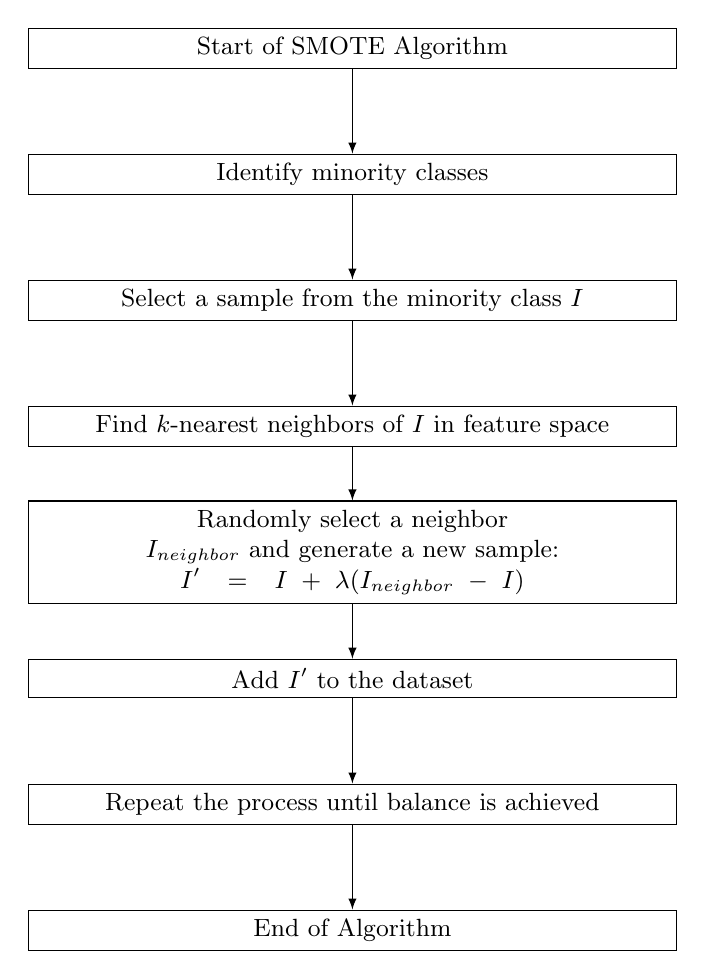
\begin{tikzpicture}[
    node distance=1.6cm,
    every node/.style={
        rectangle,
        draw,
        align=center,
        font=\small,
        text width=8cm,
    },
    >=latex, auto, font=\small
]

\node (start) {Start of SMOTE Algorithm};
\node (identify) [below of=start] {Identify minority classes};
\node (select) [below of=identify] {Select a sample from the minority class \( I \)};
\node (knn) [below of=select] {Find \( k \)-nearest neighbors of \( I \) in feature space};
\node (create) [below of=knn] {Randomly select a neighbor \( I_{\text{neighbor}} \) and generate a new sample: \\ \( I' = I + \lambda (I_{\text{neighbor}} - I) \)};
\node (add) [below of=create] {Add \( I' \) to the dataset};
\node (iterate) [below of=add] {Repeat the process until balance is achieved};
\node (end) [below of=iterate] {End of Algorithm};

\draw[->] (start) -- (identify);
\draw[->] (identify) -- (select);
\draw[->] (select) -- (knn);
\draw[->] (knn) -- (create);
\draw[->] (create) -- (add);
\draw[->] (add) -- (iterate);
\draw[->] (iterate) -- (end);

\end{tikzpicture}
\caption{فلوچارت الگوریتم SMOTE}
\label{fig:smote-flowchart}
\end{figure}
\subsection{فلوچارت وزن‌دهی در تابع هزینه}
این فلوچارت فرآیند اختصاص وزن به کلاس‌ها در تابع هزینه را برای کاهش تأثیر داده‌های نامتعادل تشریح می‌کند (شکل~\ref{fig:weighting-flowchart}).

\begin{figure}[ht]
\centering
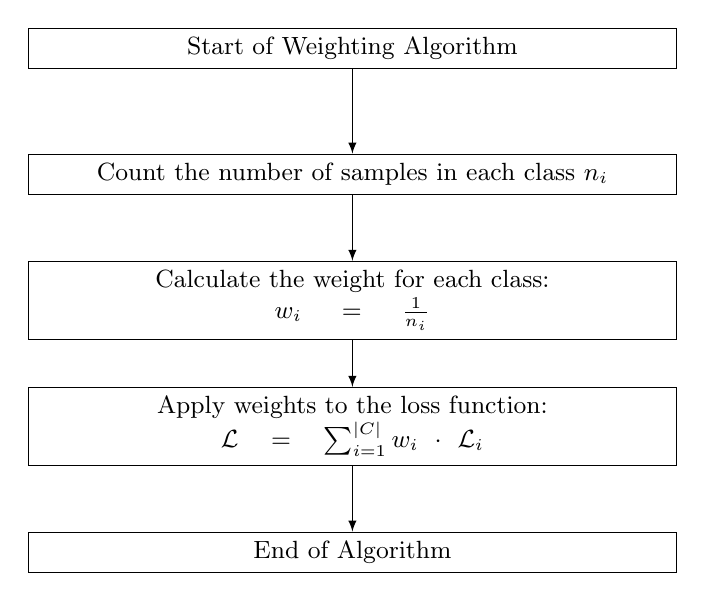
\begin{tikzpicture}[
    node distance=1.6cm,
    every node/.style={
        rectangle,
        draw,
        align=center,
        font=\small,
        text width=8cm,
    },
    >=latex, auto, font=\small
]

\node (start) {Start of Weighting Algorithm};
\node (count) [below of=start] {Count the number of samples in each class \( n_i \)};
\node (weight_calc) [below of=count] {Calculate the weight for each class: \\ \( w_i = \frac{1}{n_i} \)};
\node (apply_loss) [below of=weight_calc] {Apply weights to the loss function: \\ \( \mathcal{L} = \sum_{i=1}^{|C|} w_i \cdot \mathcal{L}_i \)};
\node (end) [below of=apply_loss] {End of Algorithm};

\draw[->] (start) -- (count);
\draw[->] (count) -- (weight_calc);
\draw[->] (weight_calc) -- (apply_loss);
\draw[->] (apply_loss) -- (end);

\end{tikzpicture}
\caption{فلوچارت وزن‌دهی در تابع هزینه}

%------------------------------------------------------------------


\label{fig:weighting-flowchart}
\end{figure}
%------------------------------------------------------------------
%   NEW SECTION (MORE PROFESSIONAL, WITH \lr{} USAGE)
%------------------------------------------------------------------

\section{مروری بر روش های افزایش داده}
در این بخش، چهار روش اصلی برای غنی‌سازی و متوازن‌سازی داده‌ها معرفی می‌گردد که در پروژهٔ حاضر تأثیر قابل‌توجهی داشته‌اند. هر یک از این روش‌ها، به‌صورت مستقل یا در ترکیب با یکدیگر، می‌تواند در سامانه‌های مختلف (از محیط‌های آزمایشگاهی تا سیستم‌های تولیدی در مقیاس وسیع) مورد استفاده قرار گیرد.

\begin{itemize}
    \item \textbf{چرخش تصادفی \lr{(Random Rotation)}:}
    با اعمال زوایای مختلف بر تصاویر ورودی، سامانه می‌تواند الگوهای چرخیدهٔ تابلوها را نیز تشخیص دهد. این روش، به‌ویژه در مواردی که تصاویر به شکل اتفاقی یا از دوربین‌هایی با زوایای غیرثابت ثبت می‌شوند، اثربخشی بالایی دارد. در سطح تولید، این فرایند اغلب قبل از ذخیره‌سازی تصاویر در دیتابیس یا هنگام آماده‌سازی ک\lr{batch}ها اعمال می‌شود تا مدل در طول آموزش با تنوع زاویه مواجه گردد.

    \item \textbf{تغییر روشنایی و کنتراست \lr{(ColorJitter)}:}
    شبیه‌سازی شرایط نوری مختلف (روز، شب، هوای ابری و غیره) کمک می‌کند مدل در سناریوهای واقعی قوی‌تر عمل کند. این روش در سامانه‌های هوشمند تشخیص علائم، خصوصاً برای دوربین‌هایی با نوردهی متغیر یا در محیط‌هایی با نور ناهمگن، بسیار مفید است. در مراکز پردازشی بزرگ (نظیر \lr{HPC} یا خوشه‌های محاسباتی)، می‌توان این فرایند را به‌صورت توزیع‌شده اعمال کرد تا عملیات پیش‌پردازش سنگین پیش از مرحلهٔ آموزش انجام شود.

    \item \textbf{\lr{SMOTE} در سطح ویژگی:}
    در مواردی که برخی کلاس‌ها (مانند نوع خاصی از علائم نادر) نمونه‌های بسیار کمی داشته باشند، مدل تمایل به نادیده‌گرفتن آن‌ها پیدا می‌کند. \lr{SMOTE} با تولید نمونه‌های مصنوعی بر اساس همسایگی داده‌های واقعی در فضای ویژگی، تنوع داده را بالا می‌برد. این الگوریتم اغلب بعد از استخراج بردار ویژگی از شبکه‌های عمیق (مثلاً لایه‌های میانی \lr{CNN}) اعمال می‌گردد تا نمونه‌های کم‌تعداد تقویت شوند. در سامانه‌های مقیاس بزرگ، اجرای \lr{SMOTE} ممکن است به‌صورت دنباله‌ای (Pipeline) با سایر مراحل تحلیل داده ادغام شود.



\begin{itemize}
    \item \textbf{وزن‌دهی در تابع هزینه\LTRfootnote{Weighted Loss}:}
    اگر توزیع کلاس‌ها بسیار نامتعادل باشد، اختصاص ضرایب وزنی بالاتر به کلاس‌های کم‌نمونه در حین آموزش (مثلاً از طریق تابع آنتروپی متقاطع\LTRfootnote{CrossEntropyLoss} وزندار) مانع از غلبهٔ کلاس‌های پرتعداد می‌شود. این تکنیک در زیرساخت‌های تولیدی\LTRfootnote{Production} نیز کاربرد زیادی دارد؛ چراکه می‌توان بدون تغییر در داده‌ها، اهمیت برخی کلاس‌ها را بیشتر کرد و مدل را به سادگی بازآموزی\LTRfootnote{Retrain} نمود.
\end{itemize}

\paragraph{روش پیاده‌سازی و نکات اجرایی:}
\begin{itemize}
    \item در کتابخانهٔ پای‌تورچ\LTRfootnote{PyTorch}، می‌توان با استفاده از ترکیب تبدیل‌ها\LTRfootnote{transforms.Compose} مجموعه‌ای از تبدیلات مانند چرخش تصادفی\LTRfootnote{RandomRotation} و تغییرات رنگ\LTRfootnote{ColorJitter} را تعریف کرد. این فرایند اغلب در مرحلهٔ بارگذار داده‌ها\LTRfootnote{DataLoader} و پیش از ارسال داده به مدل انجام می‌شود تا همهٔ عملیات لازم در حین بارگیری تصاویر صورت گیرد.
    
    \item برای بهره‌گیری از تکنیک نمونه‌برداری اقلیت مصنوعی\LTRfootnote{SMOTE (Synthetic Minority Oversampling Technique)} در فضای ویژگی، ابتدا داده‌ها را از طریق شبکهٔ اولیه یا مدل از پیش‌آموزش‌دیده\LTRfootnote{Pretrained Model} عبور داده و خروجی لایه‌های میانی را استخراج می‌کنند. سپس الگوریتم SMOTE روی این بردارهای ویژگی اعمال می‌شود تا دادهٔ مصنوعی تولید گردد. در سیستم‌های بزرگ، این مرحله ممکن است در ریزخدمات\LTRfootnote{Microservices} یا ماژول‌های جداگانه انجام پذیرد.
    
    \item در مورد وزن‌دهی در تابع هزینه\LTRfootnote{Weighted Loss}، تعیین وزن هر کلاس اغلب بر اساس معکوس فراوانی آن در مجموعهٔ آموزشی انجام می‌شود. پیاده‌سازی عملی در پای‌تورچ معمولاً از طریق متد \texttt{nn.CrossEntropyLoss(weight=\dots)} صورت می‌گیرد. این روش بدون تغییر داده‌های خام، تأکید بیشتری بر کلاس‌های کم‌نمونه دارد و در مدل‌های مستقر در محیط تولید نیز به‌آسانی به‌روزرسانی می‌شود.
\end{itemize}

\noindent
ترکیب این چهار روش—چرخش تصادفی\LTRfootnote{RandomRotation}، تغییرات رنگ\LTRfootnote{ColorJitter}، تکنیک نمونه‌برداری \texttt{SMOTE} و وزن‌دهی در تابع هزینه\LTRfootnote{Weighted Loss}—به افزایش تنوع داده و رفع مشکل عدم‌تعادل کمک می‌کند. نتیجهٔ این امر، دستیابی به مدلی است که در محیط‌های واقعی و در مواجهه با موقعیت‌های متنوع، دقت و پایداری بیشتری از خود نشان می‌دهد.


\section{معیارهای ارزیابی و مقایسه روش‌ها}

پس از اینکه داده‌هایمان را روی مدل آموزش دادیم، نیاز به ارزش‌یابی مدل و روش‌های استفاده‌شده داریم. همچنین برای مقایسه روش‌های مختلف، معیارهای ارزیابی اهمیت بسیاری دارند. در این بخش، چند مورد از معیارهای ارزیابی مدل‌ها همراه با معادل انگلیسی آن‌ها و فرمول‌ها معرفی و توضیح داده می‌شود.

دقت کلی\footnote{\lr{Accuracy}} یکی از ابتدایی‌ترین معیارها برای سنجش عملکرد مدل است که نسبت پیش‌بینی‌های صحیح مدل را صرف نظر از نوع کلاس نشان می‌دهد. این معیار برای مجموعه داده‌هایی که تعداد نمونه‌های هر کلاس تقریباً برابر است و نسبت عدم‌توازن\footnote{\lr{Imbalance Ratio}} نزدیک به \lr{1} است، یک شاخص مناسب محسوب می‌شود. با این حال، برای داده‌هایی که کلاس‌های نادر دارند، دقت کلی ممکن است تصویر اشتباهی از عملکرد مدل ارائه دهد. فرمول محاسبه نسبت عدم‌توازن و دقت کلی به شکل زیر است:

\begin{equation}
\text{\lr{Imbalance Ratio}} = \frac{\text{تعداد نمونه‌های بزرگ‌ترین کلاس}}{\text{تعداد نمونه‌های کوچک‌ترین کلاس}}
\end{equation}

\begin{equation}
\text{\lr{Accuracy}} = \frac{TP + TN}{TP + TN + FP + FN}
\end{equation}

دقت پیش‌بینی مثبت‌ها\footnote{\lr{Precision}} شاخص دیگری است که تمرکز آن بر درصد نمونه‌هایی است که به درستی به‌عنوان مثبت پیش‌بینی شده‌اند. این معیار زمانی اهمیت پیدا می‌کند که پیش‌بینی اشتباه یک کلاس مثبت هزینه بالایی داشته باشد. به عنوان مثال، در شناسایی علائم راهنمایی و رانندگی، اشتباه در پیش‌بینی علائم ایست یا سرعت می‌تواند منجر به حوادث خطرناک یا جریمه راننده شود. فرمول محاسبه این معیار به صورت زیر است:

\begin{equation}
\text{\lr{Precision}} = \frac{TP}{TP + FP}
\end{equation}

نرخ بازخوانی\footnote{\lr{Recall}} یا حساسیت، شاخصی است که توانایی مدل در شناسایی تمامی نمونه‌های مثبت واقعی را اندازه‌گیری می‌کند. این معیار در شناسایی علائم ترافیکی با اهمیت بالا، مانند علائم هشداردهنده یا محدودیت سرعت، بسیار کاربرد دارد. از دست دادن شناسایی این علائم، که به خطای منفی کاذب منجر می‌شود، می‌تواند اثرات جدی داشته باشد. فرمول محاسبه نرخ بازخوانی به شرح زیر است:

\begin{equation}
\text{\lr{Recall}} = \frac{TP}{TP + FN}
\end{equation}

امتیاز \lr{F1}\footnote{\lr{F1 Score}} به عنوان میانگین هارمونیک بین \lr{Precision} و \lr{Recall} تعریف می‌شود. این معیار به‌ویژه زمانی اهمیت پیدا می‌کند که داده‌ها نامتوازن باشند و نیاز به ارزیابی عملکرد مدل در شناسایی هر دو نوع خطای مثبت کاذب و منفی کاذب وجود داشته باشد. فرمول امتیاز \lr{F1} به شکل زیر است:

\begin{equation}
\text{\lr{F1}} = \lr{2} \times \frac{\text{\lr{Precision}} \cdot \text{\lr{Recall}}}{\text{\lr{Precision}} + \text{\lr{Recall}}}
\end{equation}

نرخ مثبت کاذب\footnote{\lr{False Positive Rate}} نشان می‌دهد که مدل چه تعداد از نمونه‌های منفی واقعی را به‌اشتباه به‌عنوان مثبت پیش‌بینی کرده است. از سوی دیگر، نرخ منفی کاذب\footnote{\lr{False Negative Rate}} مشخص می‌کند که مدل چه تعداد از نمونه‌های مثبت واقعی را نتوانسته شناسایی کند. فرمول این معیارها به صورت زیر تعریف می‌شوند:

\begin{equation}
\text{\lr{FPR}} = \frac{FP}{FP + TN}
\end{equation}

\begin{equation}
\text{\lr{FNR}} = \frac{FN}{FN + TP}
\end{equation}

منحنی \lr{ROC}\footnote{\lr{Receiver Operating Characteristic}} ارتباط بین \lr{Recall} و نرخ مثبت کاذب\footnote{\lr{False Positive Rate (FPR)}} را نمایش می‌دهد. مساحت زیر این منحنی\footnote{\lr{Area Under Curve (AUC)}} توانایی کلی مدل در تفکیک بین کلاس‌های مختلف را نشان می‌دهد. این معیار برای مدل‌هایی که احتمالات پیش‌بینی می‌کنند، مانند شبکه‌های عمیق، کاربرد ویژه‌ای دارد. فرمول محاسبه مساحت زیر منحنی \lr{ROC} به شرح زیر است:

\begin{equation}
\text{\lr{AUC}} = \int_{0}^{1} \text{\lr{ROC}}(x) dx
\end{equation}

در کنار این معیارها، ماتریس سردرگمی\footnote{\lr{Confusion Matrix}} ابزاری گرافیکی است که عملکرد مدل را با تقسیم پیش‌بینی‌ها به چهار دسته نشان می‌دهد:
\begin{figure}[h!]
\centering

\includegraphics[width=0.5\textwidth]{cof_matrix}
\caption{ماتریس سردرگمی برای مدل مورد بررسی}
\label{fig:confusion_matrix}
\end{figure}





این ماتریس برای تحلیل نقاط ضعف مدل و شناسایی کلاس‌هایی که بیشتر با یکدیگر اشتباه گرفته می‌شوند، بسیار مفید است.

در مقایسه مدل‌ها، معمولاً از ترکیبی از این معیارها استفاده می‌شود تا نقاط قوت و ضعف هر مدل به طور کامل مشخص گردد. به عنوان مثال:
\begin{itemize}
    \item مدل‌های سنتی مبتنی بر ویژگی‌های رنگ و شکل ممکن است در معیارهایی نظیر \lr{Specificity} عملکرد بهتری داشته باشند.
    \item مدل‌های یادگیری عمیق مانند شبکه‌های \lr{CNN}\footnote{\lr{Convolutional Neural Networks}} یا مدل‌های مبتنی بر \lr{Transformer}\footnote{\lr{Transformer-based Models}} معمولاً در معیارهایی نظیر \lr{AUC-ROC} و \lr{Recall} برجسته‌تر هستند.
\end{itemize}
section{مدل‌ها}
\subsection{\lr{MobileNetV2}}
\label{sec:MobileNetV2}

مدل \lr{MobileNetV2} یک شبکه عصبی کانولوشنی است که برای پردازش تصاویر طراحی شده است و به‌ویژه برای دستگاه‌های موبایل و سیستم‌های با منابع محدود بهینه‌سازی شده است. این مدل از تکنیک‌های نوینی مانند Inverted Residuals و Linear Bottlenecks بهره می‌برد که موجب کاهش پیچیدگی محاسباتی و افزایش کارایی در مقایسه با سایر مدل‌های مشابه می‌شود. از دیگر ویژگی‌های مهم این مدل، ساختار لایه‌های کانولوشنی به‌صورت Depthwise Separable Convolution است که در آن عملیات کانولوشن به دو بخش تقسیم می‌شود: کانولوشن عمقی و کانولوشن نقطه‌ای. این رویکرد باعث می‌شود که تعداد پارامترها به‌شدت کاهش یابد و در نتیجه، سرعت پردازش مدل افزایش یابد.

در مدل \lr{MobileNetV2}، به‌جای استفاده از کانولوشن‌های سنتی، از یک ساختار جدید به نام Inverted Residuals استفاده می‌شود که در آن ابتدا یک لایه‌ی عریض با تعداد فیلتر بیشتر به‌وجود می‌آید و سپس با استفاده از Linear Bottleneck به‌طور مؤثری ابعاد ویژگی کاهش می‌یابد. این رویکرد باعث می‌شود که مدل بتواند ویژگی‌های پیچیده‌تری را در لایه‌های اولیه استخراج کند و در عین حال از لحاظ محاسباتی بهینه باشد.

این مدل، برای بسیاری از کاربردهای بینایی کامپیوتری مانند شناسایی اشیاء، طبقه‌بندی تصاویر و تشخیص ویژگی‌ها در موبایل‌ها و دستگاه‌های کم‌قدرت به‌طور مؤثری مورد استفاده قرار می‌گیرد.

\begin{figure}[h!] \centering 
\includegraphics[width=0.8\textwidth]{Mobile_Fig_01} \caption{معماری شبکه عصبی \lr{MobileNetV2}} \label{fig:Mobile_Fig_01} \end{figure}

\subsection{\lr{EfficientNet}}
\label{sec:EfficientNet}

مدل \lr{EfficientNet} یکی از مدل‌های جدید و پیشرفته شبکه‌های عصبی است که توسط تیم Google AI در سال 2019 معرفی شد. این مدل به‌طور قابل توجهی نسبت به مدل‌های مشابه مانند \lr{ResNet} و \lr{MobileNet} بهینه‌تر است و برای بهبود کارایی شبکه‌های عصبی از یک رویکرد به نام Compound Scaling استفاده می‌کند. به‌عبارت دیگر، در این مدل علاوه بر افزایش عمق شبکه، مقیاس‌های دیگر مانند عرض شبکه و وضوح تصویر نیز به‌طور هم‌زمان افزایش می‌یابد تا کارایی بالاتری برای پردازش تصاویر به‌دست آید.

یکی از ویژگی‌های برجسته این مدل، کاهش Overhead در محاسبات و حافظه است. به‌طور معمول، افزایش عمق شبکه موجب افزایش میزان محاسبات و حافظه مصرفی می‌شود، اما با استفاده از رویکرد Compound Scaling در \lr{EfficientNet}، به‌طور هم‌زمان ابعاد دیگر (عرض و وضوح) به‌صورت هوشمندانه‌ای افزایش می‌یابد تا مدل بهینه‌تر و با دقت بالاتری عمل کند.

این مدل نه‌تنها تعداد پارامترها را کاهش داده، بلکه دقت بیشتری در انجام وظایف بینایی کامپیوتری ارائه می‌دهد. \lr{EfficientNet} به‌ویژه برای کار در محیط‌های با محدودیت منابع بسیار مناسب است و در بسیاری از کاربردهای پیشرفته، مانند تشخیص تصاویر در پزشکی و شناسایی اشیاء، موفقیت‌های بزرگی داشته است.

\begin{figure}[h!] \centering 
\includegraphics[width=0.8\textwidth]{EfficientNet_Fig_01} \caption{معماری \lr{EfficientNet}} \label{fig:EfficientNet_Fig_01} \end{figure}

\subsection{\lr{ResNet}} 
\label{sec:ResNet}

مدل \lr{ResNet} (\lr{Residual Networks}) یکی از موفق‌ترین و پرکاربردترین مدل‌های شبکه عصبی است که در سال 2015 توسط \lr{Kaiming He} و همکارانش معرفی شد. این مدل به‌ویژه برای شبکه‌های عمیق طراحی شده و از \lr{Residual Learning} برای حل مشکل ناپدید شدن گرادیان در شبکه‌های عصبی عمیق بهره می‌برد. یکی از مشکلات اصلی در شبکه‌های عصبی عمیق، \lr{Vanishing Gradient Problem} است که باعث می‌شود آموزش شبکه‌های با عمق زیاد بسیار دشوار و زمان‌بر شود. برای مقابله با این مشکل، \lr{ResNet} از \lr{Skip Connections} یا \lr{Residual Blocks} استفاده می‌کند که به شبکه این امکان را می‌دهد تا مسیرهای کوتاه‌تری برای جریان گرادیان‌ها داشته باشد، در نتیجه، شبکه می‌تواند به‌طور مؤثری و بدون مشکل ناپدید شدن گرادیان، آموزش ببیند.

در مدل \lr{ResNet}، از یک یا چند بلوک \lr{Residual} استفاده می‌شود که در آن ورودی هر لایه به خروجی لایه‌ی بعدی اضافه می‌شود. این روش باعث می‌شود که شبکه به راحتی به عمق‌های بیشتر گسترش یابد بدون آنکه مشکلات یادگیری ایجاد شود. این مدل در سال‌های اخیر در بسیاری از رقابت‌ها و کاربردهای بینایی کامپیوتری به موفقیت‌های زیادی دست یافته است.

\begin{figure}[h!] \centering 
\includegraphics[width=1.0\textwidth]{ResNet_Fig_01} \caption{معماری \lr{ResNet}} \label{fig:ResNet_Fig_01} \end{figure}

\subsection{ساختار معماری و اجزای اصلی}
\label{subsec:Mobile_Fig_01}

در یک نگاه کلی، ساختار مدل‌های ذکرشده را می‌توان به دو بخش اصلی تقسیم کرد:

\begin{enumerate}
    \item \textbf{بخش کانولوشنی (\lr{Convolutional Part}):}
    شبکه‌های کانولوشنی با لایه‌های مختلف و فیلترهایی در ابعاد گوناگون، به‌دنبال شناسایی ویژگی‌های موضعی در سطح فرکانس-زمان (یا هر فضای ویژگی دیگر) هستند. خروجی این بخش، معمولاً یک نگاشت ویژگی \LTRfootnote{\lr{Feature Map}} چندکاناله است که در هر مقطع زمانی، اطلاعات فشرده‌ای از الگوهای محلی \LTRfootnote{\lr{Local Patterns}} را ذخیره می‌کند.
    \item \textbf{بخش تمام‌اتصال (\lr{Fully Connected Part}):}
    پس از استخراج ویژگی‌های موضعی، معمولاً شبکه‌های عصبی به لایه‌های تمام‌اتصال یا \lr{fully connected} متصل می‌شوند تا ویژگی‌های استخراج‌شده را برای تصمیم‌گیری‌های نهایی پردازش کنند. در مدل‌هایی مانند \lr{ResNet} و \lr{MobileNetV2}، این لایه‌ها اغلب با استفاده از کلاس‌های خروجی و توابع فعال‌سازی مانند \lr{Softmax} برای طبقه‌بندی تصاویر استفاده می‌شوند.
\end{enumerate}


\subsection{مکانیزم آموزش و روش‌های ارزیابی}
\label{subsec:CNN-RNN-Training-Eval}

برای \textbf{آموزش} این مدل‌ها، ابتدا یک تابع هزینه مناسب تعریف می‌شود و سپس وزن‌های شبکه با استفاده از روش‌های بهینه‌سازی گرادیان‌محور نظیر \lr{Adam}\LTRfootnote{Adaptive Moment Estimation} یا \lr{SGD}\LTRfootnote{Stochastic Gradient Descent} به‌روزرسانی می‌گردند. بسته به این‌که مسئله از نوع طبقه‌بندی یا رگرسیون باشد، می‌توان از توابعی مانند آنتروپی متقاطع (Cross-Entropy) یا \lr{MSE}\LTRfootnote{Mean Squared Error} بهره برد. همچنین، برای جلوگیری از بیش‌برازش، روش‌هایی نظیر دراپ‌آوت \LTRfootnote{Dropout}، توقف زودهنگام \LTRfootnote{Early Stopping} و تنبیه وزن \LTRfootnote{Weight Decay} متداول هستند.

در مرحلۀ \textbf{ارزیابی} مدل، معیارهای موفقیت به نوع مسئله وابسته است: \begin{itemize} \item در سناریوهای طبقه‌بندی (مانند تشخیص اشیاء)، معیارهایی نظیر دقت \LTRfootnote{Accuracy}، امتیاز \lr{F1}\LTRfootnote{F1-Score}، \lr{Precision}\LTRfootnote{Precision} و \lr{Recall}\LTRfootnote{Recall} کاربرد دارند. \item در وظایف پیش‌بینی یا بازتولید سیگنال، معیارهایی نظیر \lr{RMSE}\LTRfootnote{Root Mean Squared Error}، \lr{MAE}\LTRfootnote{Mean Absolute Error} یا ضریب تعیین \lr{R^2}\LTRfootnote{Coefficient of Determination} به‌کار گرفته می‌شوند. \end{itemize}

ارزیابی مدل با این شاخص‌ها، میزان بهبود مدل ترکیبی را در مقایسه با روش‌های دیگر ـ یا در مقایسه با بهره‌گیری جداگانه از \lr{CNN} و \lr{RNN} ـ روشن‌تر می‌کند.        % فصل سوم: روش تحقیق

 % برای جدول‌های با عرض قابل تنظیم
   % برای استفاده از فونت‌های فارسی
% برای پشتیبانی از زبان‌های راست به چپ
% \usepackage{array}       % برای ستون‌های m{}
% \usepackage{enumitem}    % برای تنظیم فاصله لیست‌ها
% \usepackage{booktabs}    % برای خطوط زیباتر در جدول‌ها


% تعریف یک ستون m{عرض} با مرکزچین کردن افقی
\newcolumntype{M}[1]{>{\centering\arraybackslash}m{#1}}





\chapter{نتایج}

%------------------------------------------------------------------------------------------------
\section{معرفی مجموعه داده}
\subsection{ضرورت انتخاب دیتاست مناسب}
انتخاب دیتاست مناسب یکی از حیاتی‌ترین مراحل است. این انتخاب مستقیماً بر دقت و موفقیت مدل‌های یادگیری ماشین تأثیر می‌گذارد. یک دیتاست ایده‌آل باید از تنوع بالایی در شرایط محیطی برخوردار باشد؛ به عنوان مثال، شرایطی مانند نورپردازی، زاویه دید و وضوح تصاویر باید به گونه‌ای متنوع باشند که مدل بتواند عملکردی قابل قبول در محیط‌های واقعی داشته باشد.

جامعیت و تعداد نمونه‌های کافی برای هر کلاس از علائم راهنمایی و رانندگی نیز از اهمیت بالایی برخوردار است. این ویژگی به مدل امکان می‌دهد تا انواع مختلف علائم را به درستی یاد بگیرد و دقت خود را در پیش‌بینی بهبود بخشد. علاوه بر این، ساختار استاندارد دیتاست و انوتیشن‌های دقیق نظیر جعبه‌های محصور\LTRfootnote{Bounding Boxes} یا ماسک‌های تفکیکی\LTRfootnote{Segmentation Masks} می‌توانند فرآیند آموزش و ارزیابی را تسهیل کنند. پذیرش گسترده دیتاست در جامعه علمی نیز به عنوان یک شاخص کیفیت و اعتبار، انتخاب آن را برای تحقیقات تسهیل می‌کند. 

تعادل کلاس‌ها و پوشش جغرافیایی گسترده دیتاست نقش مهمی در جلوگیری از تعصب مدل به کلاس‌های پرتعداد ایفا می‌کنند. در نهایت، دسترسی آزاد و مجوزهای مناسب استفاده از دیتاست، امکان بهره‌برداری در پروژه‌های آتی را فراهم می‌کند. 

\section{بررسی و تحلیل دیتاست‌ها}

در ادامه، به بررسی و تحلیل چندین دیتاست معتبر در حوزه شناسایی علائم راهنمایی و رانندگی می‌پردازیم. هر یک از این دیتاست‌ها دارای ویژگی‌ها و کاربردهای خاص خود هستند که آن‌ها را برای پروژه‌های مختلف مناسب می‌سازد. 

دیتاست \textbf{GTSRB\LTRfootnote{German Traffic Sign Recognition Benchmark}} یکی از پرکاربردترین مجموعه داده‌ها در این زمینه است که شامل \lr{50,000} تصویر از \lr{43} کلاس مختلف علائم می‌باشد. تنوع بالای این دیتاست در شرایط نوری و زاویه دید به مدل‌ها امکان می‌دهد تا با تغییرات محیطی مختلف سازگار شوند و دقت بالایی در شناسایی علائم داشته باشند. کیفیت بالای انوتیشن‌های این دیتاست، که شامل جعبه‌های محصور است، فرآیند آموزش مدل‌ها را تسهیل کرده و دقت شناسایی را افزایش می‌دهد.

دیتاست \textbf{\lr{TT100K}\LTRfootnote{Traffic Sign Dataset 100K}} با بیش از \lr{100,000} تصویر و \lr{100} کلاس مختلف، یکی از بزرگترین دیتاست‌ها در این حوزه محسوب می‌شود. این دیتاست به دلیل تنوع بالای شرایط محیطی و تعداد زیاد نمونه‌ها برای پروژه‌هایی که نیاز به داده‌های گسترده دارند بسیار مناسب است. با این حال، تمرکز جغرافیایی این دیتاست بر روی کشور چین می‌تواند در تعمیم مدل به سایر مناطق چالش‌هایی ایجاد کند و ممکن است باعث کاهش دقت مدل‌ها در شناسایی علائم راهنمایی و رانندگی در مناطق دیگر شود.

دیتاست \textbf{LISA\LTRfootnote{Laboratory for Intelligent and Safe Automobiles}} شامل حدود \lr{25,000} تصویر از \lr{47} کلاس مختلف علائم است. این دیتاست به دلیل تعادل نسبی بین کلاس‌ها و کیفیت مناسب تصاویر، برای پروژه‌هایی که بر روی علائم در محیط‌های کنترل‌شده تمرکز دارند، بسیار مناسب است. انوتیشن‌های دقیق این دیتاست، فرآیند آموزش مدل‌ها را بهبود بخشیده و دقت شناسایی را افزایش می‌دهد.

دیتاست \textbf{Mapillary} با داشتن بیش از \lr{100,000} تصویر و \lr{600} کلاس مختلف، تنوع جغرافیایی و محیطی بسیار بالایی ارائه می‌دهد. این دیتاست برای پروژه‌های بین‌المللی و مطالعاتی که نیاز به داده‌های گسترده و متنوع دارند، گزینه‌ای ایده‌آل است. انوتیشن‌های دقیق و جامع این دیتاست، امکان آموزش مدل‌های پیچیده‌تر و دقیق‌تر را فراهم می‌آورد.

دیتاست \textbf{BelgiumTS\LTRfootnote{Belgium Traffic Sign Dataset}} شامل حدود \lr{7,000} تصویر از \lr{108} کلاس مختلف علائم است. اگرچه کیفیت تصویری بالایی دارد، اما به دلیل محدودیت در تعداد نمونه‌ها و تنوع محیطی کمتر، برای پروژه‌هایی که نیاز به تنوع و داده‌های گسترده دارند، مناسب نیست. این دیتاست بیشتر برای پروژه‌های کوچک‌تر و تحقیقات مقدماتی کاربرد دارد.


علاوه بر دیتاست‌های فوق، تکنولوژی‌های نوینی مانند \textbf{ترنسفورمر های بینایی  \LTRfootnote{Vision Transformers}} و روش‌های ترکیبی بین شبکه‌های عصبی کانولوشنی و ترنسفورمرها نیازمند دیتاست‌هایی با ساختار مناسب و ویژگی‌های دقیق هستند. دیتاست‌هایی که توانسته‌اند نیازهای این مدل‌های پیشرفته را برآورده کنند، نقش مهمی در پیشرفت تحقیقات و بهبود عملکرد سیستم‌های شناسایی علائم راهنمایی و رانندگی ایفا می‌کنند. به عنوان مثال، دیتاست‌های با انوتیشن‌های دقیق و تنوع بالا، امکان استفاده بهینه از مدل‌های ترنسفورمر را فراهم می‌آورند و باعث افزایش دقت و سرعت شناسایی می‌شوند.









\begin{latin}

\begin{table}[h!]
\centering
\resizebox{\textwidth}{!}{%
\begin{tabular}{|l|c|c|c|c|c|c|c|}
\hline
\textbf{Dataset} & \textbf{\#Images} & \textbf{\#Classes} & \textbf{\#Signs} & \textbf{Attributes} & \textbf{Region} & \textbf{BBoxes} & \textbf{Unique} \\
\hline
MTSD (TRAIN+VAL) & 41,907 & 313 & *206,388 & occluded, exterior, & \textbf{world-wide} & \checkmark & \checkmark \\
MTSD & 100,000 & 313 & 325,172 & out-of-frame, dummy, & \textbf{world-wide} & \checkmark & $\times$ \\
 &  &  &  & ambiguous, included &  &  & \\
\hline
TT100K\LTRfootnote{Traffic Sign Detection in 100K Images} & $\dagger$100,000 & $\parallel$221 & 26,349 & \textbf{--} & China & \checkmark & \checkmark \\\hline
MVD\LTRfootnote{Mapillary Vistas Dataset} & 20,000 & $\dagger$2 & 174,541 & \textbf{--} & \textbf{world-wide} & \checkmark & \checkmark \\
\hline
GTSDB\LTRfootnote{German Traffic Sign Detection Benchmark} & 900 & 43 & 852 & \textbf{--} & Germany & \checkmark & $\times$ \\\hline
RTSD\LTRfootnote{Russian Traffic Sign Dataset} & $\dagger$179,138 & 156 & $\dagger$104,358 & \textbf{--} & Russia & \checkmark & $\times$ \\\hline
STS\LTRfootnote{Swedish Traffic Signs} & 3,777 & 20 & 5,582 & \textbf{--} & Sweden & \checkmark & $\times$ \\\hline
LISA\LTRfootnote{Laboratory for Intelligent and Safe Automobiles Dataset} & 6,610 & 47 & 7,855 & \textbf{--} & USA & \checkmark & $\times$ \\
\hline
GTSRB\LTRfootnote{German Traffic Sign Recognition Benchmark} & \textbf{--} & 43 & 39,210 & \textbf{--} & Germany & $\times$ & $\times$ \\\hline
BelgiumTS\LTRfootnote{Belgium Traffic Sign Dataset} & \textbf{--} & 108 & 8,851 & \textbf{--} & Belgium & $\times$ & $\times$ \\
\hline
\end{tabular}%
}



\end{table}
\caption{
 \lr{Overview of traffic sign datasets.}
}
\end{latin}

\begin{quote}
    \textbf{
    
    جدول ۱. بررسی اجمالی دیتاست‌های علائم راهنمایی و رانندگی.} این جدول مقایسه‌ای دقیق از چندین دیتاست معتبر شناسایی علائم راهنمایی و رانندگی را ارائه می‌دهد. اعداد ذکر شده تنها شامل تصاویر و انوتیشن‌های عمومی و قابل‌دسترس هستند. ستون «منحصربه‌فرد» به دیتاست‌هایی اشاره دارد که در آن‌ها هر باکس علائم راهنمایی فقط یک نمونه منحصربه‌فرد را نمایش می‌دهد و از تکرار یک علامت در تصاویر مختلف جلوگیری شده است. $\ast$66,138 علامت درون یک تاکسونومی خاص قرار دارند. $\dagger$دیتاست \lr{TT100K} تنها شامل 10,000 تصویر از علائم راهنمایی است. $\parallel$فقط 45 کلاس از دیتاست \lr{TT100K} بیش از 100 نمونه دارند. $\dagger$دیتاست \lr{MVD} شامل تنها دو کلاس «پشت» و «جلو» است. $\ddagger$فریم‌های ویدیویی تنها 15,630 علامت منحصربه‌فرد را پوشش می‌دهند. $\S$علامت‌های موجود در مجموعه انوتیشن‌های جزئی با علامت‌های مجموعه آموزش مطابقت دارند. هر دیتاست با توجه به ویژگی‌هایی مانند پوشش جغرافیایی، جعبه‌های محصور و استانداردهای انوتیشن برای مدل‌های یادگیری ماشین در شرایط واقعی ارزیابی شده است.
    
    
\end{quote}




\begin{figure}[H]
    \centering
    % ردیف اول تصاویر
    \begin{subfigure}[b]{0.45\textwidth}
        \centering
        
\includegraphics[width=\textwidth]{GTSRB_sample} % جایگزین با نام فایل تصویر اول
        \caption{تصویر نمونه از دیتاست GTSRB}
        \label{fig:image1}
    \end{subfigure}
    \hfill
    \begin{subfigure}[b]{0.45\textwidth}
        \centering
        
\includegraphics[width=\textwidth]{TTK110_sample} % جایگزین با نام فایل تصویر دوم
        \caption{تصویر نمونه از دیتاست TT100K}
        \label{fig:image2}
    \end{subfigure}
    
    \vspace{0.5cm} % فاصله بین ردیف‌ها
    
    % ردیف دوم تصاویر
    \begin{subfigure}[b]{0.45\textwidth}
        \centering
        
\includegraphics[width=\textwidth]{Lisa_sample} % جایگزین با نام فایل تصویر سوم
        \caption{تصویر نمونه از دیتاست LISA}
        \label{fig:image3}
    \end{subfigure}
    \hfill
    \begin{subfigure}[b]{0.45\textwidth}
        \centering
        
\includegraphics[width=\textwidth]{Belgium_sample} % جایگزین با نام فایل تصویر چهارم
        
      
        \label{fig:image4}
        
    \end{subfigure}
    
    \caption{تصاویر نمونه از دیتاست‌های مختلف شناسایی علائم راهنمایی و رانندگی}
    \label{fig:dataset_samples}
\end{figure}
\clearpage



\begin{latin}
\centering
\renewcommand{\arraystretch}{1} % Increase height of cells
\tiny % Reduce the font size, you can also use \footnotesize, \scriptsize, or \tiny
\begin{longtable}{|p{2cm}|p{1.5cm}|p{2cm}|p{2cm}|p{4cm}|} % Adjust column widths
\hline
\textbf{Author/Year} & \textbf{Model} & \textbf{Dataset} & \textbf{Accuracy (\%)} & \textbf{Key Features} \\ 
\hline
Kerim and Efe (2021) & ANN & GTSRB & 95.0 & Hybrid ANN with HOG, LBP \\ 
\hline
Li et al. (2022) & Color Histogram + PCA + HOG & GTSRB & 99.99 & Dimensionality reduction with PCA and improved HOG \\ 
\hline
Zaibi et al. (2021) & LeNet-5 & GTSRB, BTSD & 99.84 (GTSRB), 98.37 (BTSD) & Enhanced LeNet-5 with dropout, batch normalization \\ 
\hline
Bangquan and Xiong (2019) & Efficient CNN & GTSRB, LISA & 98.6 & Combines VGG16 and LeNet for efficiency \\ 
\hline
Vincent et al. (2020) & CNN & GTSRB, TT100K & 98.44 & Basic CNN with data augmentation \\ 
\hline
Mishra and Goyal (2022) & CNN & GTSRB, BTSC, Mapillary & 99.76 (GTSRB), 99.79 (BTSC) & Uses advanced augmentation for robustness \\ 
\hline
Chu et al. (2023) & TRD-YOLO & TT100K, Mapillary & 99.4 (TT100K), 98.5 (Mapillary) & Optimized YOLO for small traffic sign detection \\ 
\hline
Wang et al. (2021) & YOLOv5 & TT100K, GTSRB & 99.2 (TT100K), 98.9 (GTSRB) & Real-time multi-scale detection with YOLOv5 \\ 
\hline
Mingwin et al. (2024) & Vision Transformer & GTSRB, BTSC, Mapillary & 99.85 (GTSRB), 99.9 (BTSC) & Leveraged Vision Transformers for enhanced feature extraction \\ 
\hline
\end{longtable}
\end{latin}



\begin{quote}
    \textbf{جدول ۲. مقایسه مدل‌ها و دیتاست‌های شناسایی علائم راهنمایی و رانندگی.} 
    این جدول شامل مدل‌های مختلف، دیتاست‌های استفاده‌شده، دقت آن‌ها و ویژگی‌های کلیدی برای مقایسه عملکرد و تکنیک‌های به‌کاررفته است.
\end{quote}









\subsection{دلایل انتخاب و عدم انتخاب دیتاست‌ها}

پس از بررسی و مقایسه دقیق دیتاست‌های مختلف، \lr{GTSRB} به عنوان مناسب‌ترین گزینه برای این پروژه انتخاب شد. این دیتاست به دلیل جامعیت بالا، تنوع مناسب در شرایط محیطی و کیفیت استاندارد تصاویر، امکان آموزش مدل‌هایی با قابلیت تعمیم‌پذیری بالا را فراهم می‌کند. علاوه بر این، پذیرش گسترده \lr{GTSRB} در جامعه علمی و دسترسی آزاد به آن، شرایط ایده‌آلی را برای مقایسه نتایج و استفاده عملی در تحقیقات ایجاد می‌کند.

سایر دیتاست‌ها، علی‌رغم داشتن ویژگی‌های مثبت، به دلیل محدودیت‌هایی مانند تمرکز جغرافیایی محدود، عدم تعادل در نمونه‌های کلاس‌ها، یا نیاز به منابع محاسباتی گسترده، برای اهداف این پروژه مناسب تشخیص داده نشدند. به عنوان مثال، \lr{TT100K} به دلیل تمرکز بر یک منطقه خاص و تنوع محدود در برخی کلاس‌ها، گزینه ایده‌آلی برای تعمیم مدل نبود. \lr{LISA} نیز با وجود طراحی مناسب برای محیط‌های کنترل‌شده، فاقد تنوع لازم برای استفاده در شرایط واقعی بود. همچنین، پیچیدگی انوتیشن‌ها در \lr{Mapillary} و تعداد محدود نمونه‌ها در \lr{BelgiumTS} استفاده از این دیتاست‌ها را برای پروژه‌ای با نیاز به داده‌های متنوع و گسترده دشوار می‌کرد.


. \begin{figure}[H]
    \centering
    
\includegraphics[width=1\textwidth]{all_classes_sample}
    \caption{
    نمونه های موجود در هر کلاس در مجموعه داده ،}
    
    \label{fig: sample_ditribution}
\end{figure}


%------------------------------------------------------------------------------------------------
%------------------------------------------------------------------------------------------------
\section{تحلیل ویژگی های آماری }
علائم راهنمایی و رانندگی به‌گونه‌ای طراحی شده‌اند که برای انسان‌ها قابل‌فهم و سریعاً قابل‌تشخیص باشند. در این طراحی، از تأثیر شکل‌ها و رنگ‌های مختلف بر ادراک انسانی بهره گرفته شده است تا پیام‌ها به ساده‌ترین و مؤثرترین شکل منتقل شوند. به عنوان مثال، رنگ قرمز که به طور طبیعی حس هشدار یا توقف را القا می‌کند، برای علائم ممنوعیت یا ایست استفاده می‌شود، و شکل مثلث که توجه را جلب می‌کند، برای علائم هشداردهنده به کار می‌رود.

در تحلیل آماری دیتاست علائم راهنمایی و رانندگی، دسته‌بندی داده‌ها نقش کلیدی در درک ساختار و ویژگی‌های آن دارد. این دیتاست شامل ۴۳ کلاس است که هر کدام نشان‌دهنده یک علامت خاص با معنا و کاربرد مشخص است. برای تحلیل جامع‌تر، داده‌ها را می‌توان از جنبه‌های مختلفی مانند معنایی، بصری و پیچیدگی دسته‌بندی کرد. هر یک از این دسته‌بندی‌ها دیدگاه متفاوتی را ارائه می‌دهد و به ما کمک می‌کند تا الگوها و ارتباطات پنهان در داده‌ها را کشف کنیم.

در این پروژه، ما با دسته‌بندی علائم بر اساس ویژگی‌های بصری مانند رنگ، شکل و پیچیدگی، و همچنین گروه‌بندی مفاهیم علائم به دسته زیردسته‌ها، تلاش می‌کنیم تا مدل را به درکی نزدیک به ادراک انسانی برسانیم. هدف این است که مدل نه تنها توانایی شناسایی و تشخیص علائم را داشته باشد، بلکه بتواند مفهوم آن‌ها را درک کرده و واکنشی مشابه رفتار انسان در مواجهه با این علائم نشان دهد. این رویکرد، پایه‌ای برای تحلیل دقیق‌تر توزیع داده‌ها و توسعه مدل‌هایی است که به طور طبیعی‌تر و مؤثرتر با محیط‌های واقعی تعامل داشته باشند. در ادامه، جزئیات هر دسته‌بندی و تأثیر آن بر عملکرد مدل مورد بررسی قرار خواهد گرفت.

\subsection{دسته بندی معنایی و بصری}


علائم راهنمایی و رانندگی را طی یک فرآیند دو مرحله‌ای دسته‌بندی کردیم تا درک عمیق‌تری از معنای علائم و ویژگی‌های بصری آن‌ها به دست آوریم. در مرحله اول، علائم را بر اساس مفهوم و کاربردشان، بدون توجه به رنگ و شکل، گروه‌بندی کردیم. این مرحله با بهره‌گیری از تحلیل معنایی انجام شد تا معنا و نقش عملکردی علائم در مدیریت ترافیک بررسی شود. در مرحله دوم، علائم را با توجه به ویژگی‌های بصری مانند رنگ و شکل دسته‌بندی کردیم. در این بخش از اصول روان‌فیزیک استفاده کردیم تا نحوه ادراک علائم توسط انسان‌ها و ارتباط میان طراحی فیزیکی علائم و پیام آن‌ها را تحلیل کنیم. با ترکیب این دو رویکرد، مدلی طراحی کردیم که نه تنها توانایی شناسایی علائم را دارد، بلکه می‌تواند مفهوم و عملکرد آن‌ها را نیز درک کند. این روش دوگانه، توانایی مدل در تصمیم‌گیری آگاهانه‌تر و شبیه‌تر به انسان را بهبود بخشید و گامی مهم در نزدیک‌تر کردن عملکرد هوش مصنوعی به ادراک انسانی بود.


% Define centered m{} column type
\newcolumntype{M}[1]{>{\centering\arraybackslash}m{#1}}
\begin{table}[htbp]
    \centering
    \renewcommand{\arraystretch}{0.6}
    \setlength{\tabcolsep}{4pt}      
    \resizebox{\textwidth}{!}{        % Scale table to fit page width
        \begin{tabular}{|M{4cm}|M{4cm}|M{8cm}|} % Centered columns
        \hline
        \textbf{دسته اصلی} & \textbf{زیردسته} & \textbf{تصاویر کلاس‌ها} \\ \hline
        \multirow{3}{*}{علائم محدودیت سرعت} 
        & سرعت پایین & 
        
\includegraphics[width=1cm]{0} \hspace{0.1cm}
        
\includegraphics[width=1cm]{1} \hspace{0.1cm}
        
\includegraphics[width=1cm]{2} \\ \cline{2-3}
        & سرعت متوسط & 
        
\includegraphics[width=1cm]{3} \hspace{0.1cm}
        
\includegraphics[width=1cm]{4} \hspace{0.1cm}
        
\includegraphics[width=1cm]{5} \\ \cline{2-3}
        & سرعت بالا & 
        
\includegraphics[width=1cm]{7} \hspace{0.1cm}
        
\includegraphics[width=1cm]{8} \\ \hline
        \multirow{2}{*}{علائم ممنوعیت دیگر} 
        & محدودیت‌های وسیله نقلیه & 
        
\includegraphics[width=1cm]{9} \hspace{0.1cm}
        
\includegraphics[width=1cm]{10} \\ \cline{2-3}
        & ممنوعیت‌های عمومی & 
        
\includegraphics[width=1cm]{15} \hspace{0.1cm}
        
\includegraphics[width=1cm]{16} \\ \hline
        \multirow{2}{*}{علائم رفع محدودیت} 
        & رفع محدودیت سرعت & 
        
\includegraphics[width=1cm]{6} \hspace{0.1cm}
        
\includegraphics[width=1cm]{32} \\ \cline{2-3}
        & رفع محدودیت سبقت & 
        
\includegraphics[width=1cm]{41} \hspace{0.1cm}
        
\includegraphics[width=1cm]{42} \\ \hline
        \multirow{2}{*}{علائم اجباری} 
        & علائم جهت‌دهی اولیه & 
        
\includegraphics[width=1cm]{33} \hspace{0.1cm}
        
\includegraphics[width=1cm]{34} \hspace{0.1cm}
        
\includegraphics[width=1cm]{35} \\ \cline{2-3}
        & علائم جهت‌دهی ثانویه & 
        
\includegraphics[width=1cm]{36} \hspace{0.1cm}
        
\includegraphics[width=1cm]{37} \hspace{0.1cm}
        
\includegraphics[width=1cm]{38} \hspace{0.1cm}
        
\includegraphics[width=1cm]{39} \\ \hline
        \multirow{6}{*}{علائم خطر} 
        & هشدارهای عمومی & 
        
\includegraphics[width=1cm]{18} \hspace{0.1cm}
        
\includegraphics[width=1cm]{30} \\ \cline{2-3}
        & خطرات هندسی جاده & 
        
\includegraphics[width=1cm]{24} \hspace{0.1cm}
        
\includegraphics[width=1cm]{23} \hspace{0.1cm}
        
\includegraphics[width=1cm]{20} \hspace{0.1cm}
        
\includegraphics[width=1cm]{19} \\ \cline{2-3}
        & شرایط سرعت و سطح جاده & 
        
\includegraphics[width=1cm]{22} \hspace{0.1cm}
        
\includegraphics[width=1cm]{29} \\ \cline{2-3}
        & خطرات ترافیک و عابر پیاده & 
        
\includegraphics[width=1cm]{28} \hspace{0.1cm}
        
\includegraphics[width=1cm]{27} \hspace{0.1cm}
        
\includegraphics[width=1cm]{26} \hspace{0.1cm}
        
\includegraphics[width=1cm]{25} \\ \cline{2-3}
        & خطرات محیطی & 
        
\includegraphics[width=1cm]{31} \hspace{0.1cm}
        
\includegraphics[width=1cm]{11} \\ \cline{2-3}
        & مناطق کار و ساخت‌وساز & 
        
\includegraphics[width=1cm]{21} \\ \hline
        \multirow{3}{*}{علائم خاص} 
        & علائم اولویت و توقف & 
        
\includegraphics[width=1cm]{13} \hspace{0.1cm}
        
\includegraphics[width=1cm]{14} \\ \cline{2-3}
        & علائم هشدار & 
        
\includegraphics[width=1cm]{12} \\ \cline{2-3}
        & ممنوعیت‌ها و محدودیت‌ها & 
        
\includegraphics[width=1cm]{17} \\ \hline
    \end{tabular}
    }
     \caption{دسته‌بندی: دسته‌ها و زیردسته‌ها مفهوم و کاربرد خاص علائم را نشان می‌دهند. هر دسته به نوعی درجه اهمیت علائم را نیز مشخص می‌کند، مانند علائم هشداردهنده برای خطرات، محدودیت‌ها برای کنترل، و دستورات برای راهنمایی مستقیم. این ساختار به درک بهتر اولویت و معنای علائم کمک می‌کند.}

    \label{tab:optimized_traffic_sign_images}
\end{table}

\clearpage
\vspace{-1cm}
\newcolumntype{M}[1]{>{\centering\arraybackslash}m{#1}}
\begin{table}[h]
    \centering
    \renewcommand{\arraystretch}{0.6}
    \setlength{\tabcolsep}{4pt}      
    \resizebox{\textwidth}{!}{        
        \begin{tabular}{|M{4cm}|M{4cm}|M{8cm}|} 
        \hline
        \textbf{رنگ} & \textbf{زیردسته} & \textbf{تصاویر کلاس‌ها} \\ \hline
        \multirow{3}{*}{قرمز و سفید} 
        & محدودیت‌ها & 
        
\includegraphics[width=1cm]{0} \hspace{0.1cm}
        
\includegraphics[width=1cm]{1} \hspace{0.1cm}
        
\includegraphics[width=1cm]{2} \hspace{0.1cm}
        
\includegraphics[width=1cm]{3} \hspace{0.1cm}
        
\includegraphics[width=1cm]{4} \hspace{0.1cm}
        
\includegraphics[width=1cm]{5} \hspace{0.1cm}
        
\includegraphics[width=1cm]{7} \hspace{0.1cm}
        
\includegraphics[width=1cm]{8} \\ \cline{2-3}
        & ممنوعیت‌ها & 
        
\includegraphics[width=1cm]{9} \hspace{0.1cm}
        
\includegraphics[width=1cm]{10} \hspace{0.1cm}
        
\includegraphics[width=1cm]{11} \hspace{0.1cm}
        
\includegraphics[width=1cm]{13} \hspace{0.1cm}
        
\includegraphics[width=1cm]{14} \hspace{0.1cm}
        
\includegraphics[width=1cm]{15} \hspace{0.1cm}
        
\includegraphics[width=1cm]{16} \hspace{0.1cm}
        
\includegraphics[width=1cm]{17} \\ \cline{2-3}
        & هشدارها & 
        
\includegraphics[width=1cm]{18} \hspace{0.1cm}
        
\includegraphics[width=1cm]{19} \hspace{0.1cm}
        
\includegraphics[width=1cm]{20} \hspace{0.1cm}
        
\includegraphics[width=1cm]{21} \hspace{0.1cm}
        
\includegraphics[width=1cm]{23} \hspace{0.1cm}
        
\includegraphics[width=1cm]{24} \hspace{0.1cm}
        
\includegraphics[width=1cm]{26} \hspace{0.1cm}
        
\includegraphics[width=1cm]{27} \hspace{0.1cm}
        
\includegraphics[width=1cm]{28} \hspace{0.1cm}
        
\includegraphics[width=1cm]{29} \hspace{0.1cm}
        
\includegraphics[width=1cm]{30} \\ \hline
        \multirow{2}{*}{سیاه و سفید} 
        & رفع محدودیت‌ها & 
        
\includegraphics[width=1cm]{6} \hspace{0.1cm}
        
\includegraphics[width=1cm]{32} \\ \cline{2-3}
        & ممنوعیت‌ها & 
        
\includegraphics[width=1cm]{41} \hspace{0.1cm}
        
\includegraphics[width=1cm]{42} \\ \hline
        زرد و سیاه & هشدارها & 
        
\includegraphics[width=1cm]{22} \hspace{0.1cm}
        
\includegraphics[width=1cm]{25} \\ \hline
        زرد و سفید & هشدارها & 
        
\includegraphics[width=1cm]{12} \\ \hline
        آبی و سفید & اطلاعاتی & 
        
\includegraphics[width=1cm]{33} \hspace{0.1cm}
        
\includegraphics[width=1cm]{34} \hspace{0.1cm}
        
\includegraphics[width=1cm]{35} \hspace{0.1cm}
        
\includegraphics[width=1cm]{36} \hspace{0.1cm}
        
\includegraphics[width=1cm]{37} \hspace{0.1cm}
        
\includegraphics[width=1cm]{38} \hspace{0.1cm}
        
\includegraphics[width=1cm]{39} \hspace{0.1cm}
        
\includegraphics[width=1cm]{40} \\ \hline
    \end{tabular}
    }
     \caption{دسته‌بندی علائم  براساس رنگ:  نقش رنگ‌ها را در انتقال معنا و مفهوم علائم بضوح قابل مشاهده است. هر رنگ با هدف خاصی طراحی شده است؛ مانند قرمز برای هشدار یا توقف، آبی برای دستورات، و زرد برای هشدارهای محیطی. این ارتباط میان رنگ و مفهوم، به درک سریع‌تر و تصمیم‌گیری بهتر کمک می‌کند.}

    \label{tab:traffic_signs_by_color}
\clearpage
\vspace{-1cm}
\end{table}
\begin{table}[h]
    \centering
    \renewcommand{\arraystretch}{0.6}
    \setlength{\tabcolsep}{4pt}      
    \resizebox{\textwidth}{!}{        
        \begin{tabular}{|M{4cm}|M{4cm}|M{8cm}|} 
        \hline
        \textbf{شکل} & \textbf{زیردسته} & \textbf{تصاویر کلاس‌ها} \\ \hline
        \multirow{3}{*}{دایره‌ای} 
        & محدودیت‌ها & 
        
\includegraphics[width=1cm]{0} \hspace{0.1cm}
        
\includegraphics[width=1cm]{1} \hspace{0.1cm}
        
\includegraphics[width=1cm]{2} \hspace{0.1cm}
        
\includegraphics[width=1cm]{3} \hspace{0.1cm}
        
\includegraphics[width=1cm]{4} \hspace{0.1cm}
        
\includegraphics[width=1cm]{5} \hspace{0.1cm}
        
\includegraphics[width=1cm]{7} \hspace{0.1cm}
        
\includegraphics[width=1cm]{8} \\ \cline{2-3}
        & ممنوعیت‌ها & 
        
\includegraphics[width=1cm]{9} \hspace{0.1cm}
        
\includegraphics[width=1cm]{10} \hspace{0.1cm}
        
\includegraphics[width=1cm]{15} \hspace{0.1cm}
        
\includegraphics[width=1cm]{16} \hspace{0.1cm}
        
\includegraphics[width=1cm]{17} \hspace{0.1cm}
        
\includegraphics[width=1cm]{32} \hspace{0.1cm}
        
\includegraphics[width=1cm]{41} \hspace{0.1cm}
        
\includegraphics[width=1cm]{42} \\ \cline{2-3}
        & اطلاعاتی & 
        
\includegraphics[width=1cm]{33} \hspace{0.1cm}
        
\includegraphics[width=1cm]{34} \hspace{0.1cm}
        
\includegraphics[width=1cm]{35} \hspace{0.1cm}
        
\includegraphics[width=1cm]{36} \hspace{0.1cm}
        
\includegraphics[width=1cm]{37} \hspace{0.1cm}
        
\includegraphics[width=1cm]{38} \hspace{0.1cm}
        
\includegraphics[width=1cm]{39} \hspace{0.1cm}
        
\includegraphics[width=1cm]{40} \\ \hline
        \multirow{2}{*}{مثلثی} 
        & هشدارها & 
        
\includegraphics[width=1cm]{11} \hspace{0.1cm}
        
\includegraphics[width=1cm]{18} \hspace{0.1cm}
        
\includegraphics[width=1cm]{19} \hspace{0.1cm}
        
\includegraphics[width=1cm]{20} \hspace{0.1cm}
        
\includegraphics[width=1cm]{21} \hspace{0.1cm}
        
\includegraphics[width=1cm]{22} \hspace{0.1cm}
        
\includegraphics[width=1cm]{23} \hspace{0.1cm}
        
\includegraphics[width=1cm]{24} \hspace{0.1cm}
        
\includegraphics[width=1cm]{25} \hspace{0.1cm}
        
\includegraphics[width=1cm]{26} \hspace{0.1cm}
        
\includegraphics[width=1cm]{27} \hspace{0.1cm}
        
\includegraphics[width=1cm]{28} \hspace{0.1cm}
        
\includegraphics[width=1cm]{29} \hspace{0.1cm}
        
\includegraphics[width=1cm]{30} \hspace{0.1cm}
        
\includegraphics[width=1cm]{31} \\ \hline
        لوزی & هشدارها & 
        
\includegraphics[width=1cm]{12} \\ \hline
        مثلث برعکس & حق تقدم & 
        
\includegraphics[width=1cm]{13} \\ \hline
        شش‌ضلعی & توقف & 
        
\includegraphics[width=1cm]{14} \\ \hline
    \end{tabular}
    }
    
\caption{دسته‌بندی علائم بر اساس شکل: این دسته‌بندی تأثیر شکل‌ها در انتقال معنا و مفهوم علائم را نشان می‌دهد.  برای مثال مثلث برای هشدار، دایره برای محدودیت‌ها، و مربع برای اطلاعات عمومی. ترکیب شکل‌ها با رنگ‌ها معنای دقیق‌تری را منتقل می‌کند، مانند مثلث قرمز برای هشدار خطر یا دایره آبی برای دستورات، که به شناسایی سریع‌تر و تصمیم‌گیری آگاهانه‌تر کمک می‌کند.}

    \label{tab:traffic_signs_by_shape}
\end{table}
\clearpage
\vspace{-1cm}


\subsection{تحلیل تنوع و عدم تعادل داده‌ها}حال برای بررسی میزان تنوع و پراکندگی داده ها ، رویکرد های متفاوتی وجود خواهد داشت، در ساده ترین حالت میتوان مجموعه داده را که متشکل از کلاس ها که هر کدام نشان دهنده یک علامت و معنا و مفهوم مستقل اند در نظر گرفت.
\subsubsection{نمودار توزیع نمونه‌ها در کلاس‌ها}
\begin{figure}[H]
    \centering
    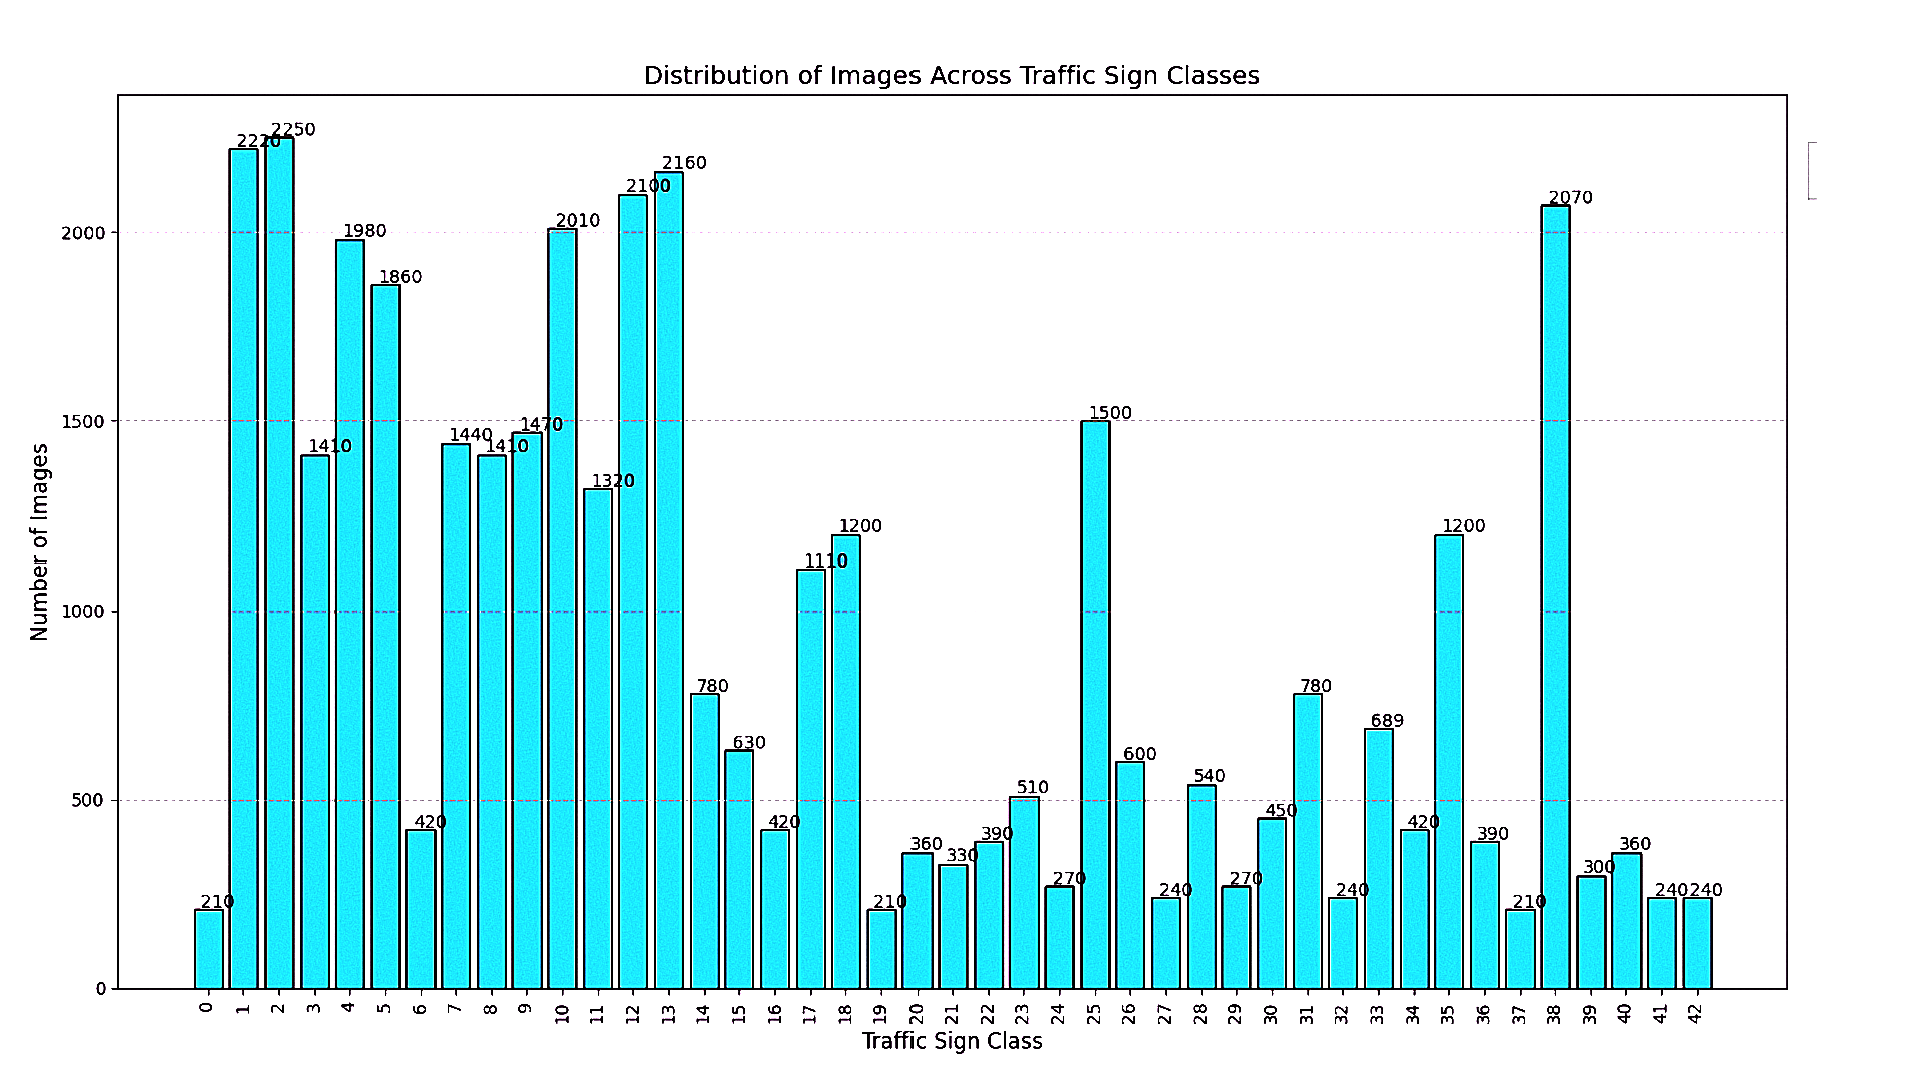
\includegraphics[width=1.2\textwidth]{bar_chart_unsorted}
    \caption{توزیع تعداد نمونه‌ها در کلاس‌ها (مرتب نشده) – این نمودار تعداد نمونه‌های موجود در هر کلاس را به ترتیب شماره کلاس‌ها (از 0 تا 42) نمایش می‌دهد. }
    \label{fig:class_dist_freq}
\end{figure}
\begin{figure}[H]
    \centering
    
\includegraphics[width=1\textwidth]{bar_chart_sorted}
    \caption{توزیع تعداد نمونه‌ها در کلاس‌ها (مرتب شده بر اساس تعداد) – در این نمودار، کلاس‌ها بر اساس تعداد نمونه‌های موجود مرتب شده‌اند تا توزیع داده‌ها به شکل واضح‌تری قابل مشاهده باشد.  }
    \label{fig:class_dist_freq}
\end{figure}











\subsubsection{تحلیل عدم تعادل داده‌ها}
اما همانطور که در بالا اشاره کردیم شیوه طراحی بصری علائم باعث شده که علائمی که شبیه هم هستند از لحاظ دسته بندی موضوعی هم بهم نزدیک تر باشند.پس می توانیم علائم را براساس معنا و جنس پیامی که انتقال می دهند که به نوعی هم میزان مهم بودن آن را نشان میدهد در زیر توزیع نمونه ها در دسته بندی های بصری و مفهومی که قبلا مطرح شد مشاهده می‌شود، توزیع نمونه‌ها در دسته‌بندی‌های مختلف از جمله رنگ، شکل، ترکیب شکل و رنگ و مفهوم علائم به وضوح نامتعادل است. این عدم توازن نشان‌دهنده فراوانی بسیار زیاد برخی دسته‌ها، مانند قرمز و سفید یا دایره، و فراوانی بسیار کم در دسته‌هایی مانند زرد و سفید با لوزی یا شش‌ضلعی است. چنین توزیعی می‌تواند مشکلات متعددی را ایجاد کند، از جمله سوگیری به سمت کلاس‌های پرتکرار، کاهش دقت در شناسایی کلاس‌های کم‌نمونه، و افت عملکرد مدل بر اساس معیارهای ارزیابی
 مانند \lr{Recall}\LTRfootnote{\lr{Recall}} و \lr{F1-Score}\LTRfootnote{\lr{F1-Score}}.

برای رفع این چالش‌ها، در این پژوهش مجموعه‌ای از تکنیک‌های افزایش داده و متوازن‌سازی به کار گرفته شده است. یکی از این تکنیک‌ها چرخش تصادفی\LTRfootnote{\lr{Random Rotation}} است که با اعمال زوایای مختلف بر تصاویر ورودی، مدل را قادر می‌سازد الگوهای چرخیده را نیز شناسایی کند. این روش با افزایش تنوع در مجموعه داده، به بهبود تعمیم‌پذیری مدل کمک کرده است. علاوه بر این، تغییر روشنایی و کنتراست\LTRfootnote{\lr{Color Jitter}} برای شبیه‌سازی شرایط نوری مختلف، مانند نور روز، شب و شرایط با روشنایی متغیر، به کار گرفته شده است. این تکنیک، مدل را در برابر تغییرات نوری مقاوم‌تر ساخته و دقت آن را در سناریوهای متنوع افزایش داده است.

همچنین، از تکنیک SMOTE\LTRfootnote{\lr{Synthetic Minority Over-sampling Technique}} برای تولید نمونه‌های مصنوعی در کلاس‌های کم‌نمونه استفاده شده است. این روش با افزایش تعداد نمونه‌های کلاس‌های نادر، توازن داده‌ها را بهبود بخشیده و شناسایی این کلاس‌ها را برای مدل تسهیل کرده است. علاوه بر این، وزن‌دهی در تابع هزینه\LTRfootnote{\lr{Weighted Loss}} نیز برای کاهش تأثیر کلاس‌های پرتکرار مورد استفاده قرار گرفته است. این تکنیک با اختصاص وزن‌های بالاتر به کلاس‌های کم‌نمونه در حین آموزش، مدل را به طور ضمنی به شناسایی این کلاس‌ها ترغیب کرده و عملکرد آن را در پیش‌بینی کلاس‌های نادر ارتقا داده است.

ترکیب این روش‌ها به افزایش تنوع داده‌ها و بهبود توازن میان کلاس‌ها منجر شده است. نتایج حاصل نشان می‌دهد که این استراتژی‌ها توانسته‌اند بر مشکلات ناشی از نامتوازن بودن داده‌ها غلبه کرده و مدلی پایدارتر، قابل‌اعتمادتر و با توانایی تعمیم بالاتر در مواجهه با داده‌های واقعی ارائه دهند. این رویکرد در مسائل عملی، به ویژه در کاربردهایی که عدم توازن داده‌ها می‌تواند به عملکرد مدل آسیب برساند


. \begin{figure}[H]
    \centering
    
\includegraphics[width=1\textwidth]{sample_ditribution}
    \caption{ این مجموعه نمودارها، توزیع نمونه‌ها را بر اساس رنگ، شکل، ترکیب شکل و رنگ و مفهوم علائم نمایش می‌دهد. نمودارها به وضوح نامتعادلی در توزیع داده‌ها را نشان می‌دهند؛ به‌طوری‌که برخی دسته‌ها مانند قرمز و سفید یا دایره بیشترین نمونه‌ها را دارند، در حالی که دسته‌هایی مانند زرد و سفید با لوزی یا شش‌ضلعی به‌ندرت دیده می‌شوند}
    \label{fig: sample_ditribution}
\end{figure}


. \begin{figure}[H]
    \centering
    
\includegraphics[width=1\textwidth]{cocept_based percentage}
    \caption{ نمودارها توزیع زیرکلاس‌های دسته‌بندی مفهومی را نمایش می‌دهند. نمودار بالا درصد نمونه‌های هر زیرکلاس را نسبت به کتگوری اصلی خود نشان می‌دهد، در حالی که نمودار پایین درصد نمونه‌های هر زیرکلاس را نسبت به کل دیتاست مقایسه می‌کند. این تحلیل به وضوح نامتوازن بودن برخی زیرکلاس‌ها را در هر دو
    مقیاس نشان می‌دهد،}
    \label{fig: cocept_based percentage}
\end{figure}
\section{متعادل‌سازی داده‌ها با استفاده از تکنیک‌های افزایش داده}

برای رفع عدم توازن در توزیع کلاس‌ها، از روش‌های افزایش داده مانند \lr{SMOTE}\LTRfootnote{Synthetic Minority Over-sampling Technique} استفاده شد. این روش با تولید نمونه‌های مصنوعی، داده‌های کلاس‌های اقلیت را افزایش داده و توزیع را متعادل می‌کند. علاوه بر آن، تکنیک‌های دیگری شامل چرخش\LTRfootnote{Rotation}، تغییر نور و روشنایی\LTRfootnote{Brightness Adjustment}، جابجایی\LTRfootnote{Translation}، افزودن نویز\LTRfootnote{Adding Noise} و تغییر مقیاس\LTRfootnote{Scaling} به کار گرفته شدند. 

این اقدامات منجر به بهبود توزیع کلاس‌ها و افزایش تنوع ویژگی‌ها شد. نتایج نشان داد که مدل پس از اعمال این روش‌ها دقت بیشتری در پیش‌بینی داده‌های اقلیت داشته و توانایی آن در مواجهه با شرایط مختلف افزایش یافته است. استفاده از این تکنیک‌ها به وضوح توانست عدم توازن داده‌ها را کاهش داده و کارایی مدل را بهبود بخشد.


\begin{figure}[H]
    \centering
    \begin{subfigure}{0.3\textwidth}
        
\includegraphics[width=\linewidth]{sample_augmented_1}
        \caption{نمونه 1}
    \end{subfigure}
    \begin{subfigure}{0.3\textwidth}
        
\includegraphics[width=\linewidth]{sample_augmented_2}
        \caption{نمونه 2}
    \end{subfigure}
    
    \caption{نمونه‌هایی از تصاویر افزوده شده}
    \label{fig:augmented_samples}
\end{figure}

همچنین، نمودار زیر توزیع کلاس‌ها را قبل و بعد از افزایش داده مقایسه می‌کند.

\begin{figure}[H]
    \centering
    
\includegraphics[width=1\textwidth]{class_distribution_comparison}
    \caption{توزیع کلاس‌ها قبل و بعد از افزایش داده}
    \label{fig:class_distribution}
\end{figure}



\begin{table}[h]
\centering
\renewcommand{\arraystretch}{1} % تنظیم فاصله عمودی سلول‌ها
\setlength{\tabcolsep}{8pt}      % تنظیم فاصله افقی سلول‌ها
\begin{tabular}{|l|l|l|}
\hline
\textbf{آمار}                                  & \textbf{قبل از افزایش داده}                      & \textbf{بعد از افزایش داده}                    \\ \hline
\lr{Max Image Count}                          & \lr{2250}                                      & \lr{2250}                                      \\ \hline
\lr{Min Image Count}                          & \lr{210}                                       & \lr{2250}                                      \\ \hline
\lr{Imbalance Ratio (Max / Min)}             & \lr{10.71}                                    & \lr{1.00}                                     \\ \hline
\lr{Average Image Count per Class}           & \lr{1036.58}                                  & \lr{2250.00}                                  \\ \hline
\lr{Standard Deviation of Image Count}       & \lr{790.44}                                   & \lr{0.00}                                     \\ \hline
\end{tabular}
\caption{ویژگی های آماری تصاویر قبل و بعد از افزایش داده در سطح کلاس}
\label{tab:statistics}
\end{table}

برای توازن داده‌ها از تکنیک‌هایی نظیر چرخش تصادفی، انتقال، وارونگی افقی و
تکنیک‌های افزایش داده به طور مؤثری داده‌ها را متوازن کرده و نسبت عدم توازن را از \lr{10.71} به \lr{1.00} کاهش داده‌اند. این امر باعث می‌شود مدل آموزش‌دیده بر روی این داده‌ها کمتر به کلاس‌هایی با تعداد بیشتر تصاویر گرایش داشته باشد.
\subsection{متعادل‌سازی در سطح دسته‌بندی‌های معنایی و بصری}

برای بهبود تعادل داده‌ها، فرآیند تعادل‌سازی نه تنها در سطح کلاس‌ها، بلکه در سطح دسته‌بندی‌های اصلی و زیرمجموعه‌های معنایی و بصری اعمال گردید. 

جدول \ref{tab:comparison} تعداد تصاویر قبل و بعد از افزایش داده را بر اساس دسته‌بندی‌های اصلی شامل رنگ، شکل و مفهوم مقایسه می‌کند. این جدول نشان‌دهنده تغییرات در توزیع داده‌ها بین این دسته‌بندی‌ها است. 

در ادامه، جدول \ref{tab:combined_ratios} به صورت جزئی‌تر به بررسی نسبت‌های عدم تعادل در زیرگروه‌های مفهومی می‌پردازد و تغییرات پیش و پس از افزایش داده را برای این زیرگروه‌ها نشان می‌دهد. این مقایسه به وضوح میزان تأثیر فرآیند افزایش داده در متعادل‌سازی زیرگروه‌های مفهومی را مشخص می‌کند.


\begin{table}[h!]
\centering
\renewcommand{\arraystretch}{0.8} % Reduce row height
\scriptsize % Reduce font size
\resizebox{\textwidth}{!}{%
\begin{tabular}{|p{4cm}|p{3cm}|p{3cm}|}
\hline
\textbf{دسته‌بندی} & \textbf{قبل از افزوده‌سازی} & \textbf{بعد از افزوده‌سازی} \\ \hline
\multicolumn{3}{|c|}{\textbf{دسته‌بندی‌های مبتنی بر رنگ}} \\ \hline
زیرگروه قرمز و سفید & \lr{10.71} & \lr{1.66} \\ \hline
زیرگروه سیاه و سفید & \lr{1.75} & \lr{1.02} \\ \hline
زیرگروه زرد و سیاه & \lr{3.85} & \lr{1.21} \\ \hline
زیرگروه زرد و سفید & \lr{1.00} & \lr{1.00} \\ \hline
زیرگروه آبی و سفید & \lr{9.86} & \lr{1.33} \\ \hline
\multicolumn{3}{|c|}{\textbf{دسته‌بندی‌های مبتنی بر شکل}} \\ \hline
زیرگروه دایره & \lr{10.71} & \lr{1.96} \\ \hline
زیرگروه مثلث & \lr{7.14} & \lr{1.29} \\ \hline
زیرگروه لوزی & \lr{1.00} & \lr{1.00} \\ \hline
زیرگروه مثلث وارونه & \lr{1.00} & \lr{1.00} \\ \hline
زیرگروه شش‌ضلعی & \lr{1.00} & \lr{1.00} \\ \hline
\multicolumn{3}{|c|}{\textbf{دسته‌بندی‌های مبتنی بر مفهوم}} \\ \hline
زیرگروه علائم محدودیت سرعت & \lr{10.71} & \lr{1.59} \\ \hline
زیرگروه علائم بازدارنده دیگر & \lr{4.79} & \lr{1.21} \\ \hline
زیرگروه علائم رفع محدودیت & \lr{1.75} & \lr{1.02} \\ \hline
زیرگروه علائم اجباری & \lr{9.86} & \lr{1.33} \\ \hline
زیرگروه علائم خطر & \lr{7.14} & \lr{1.29} \\ \hline
زیرگروه علائم منحصربه‌فرد & \lr{2.77} & \lr{1.25} \\ \hline
\end{tabular}}
\caption{جدول مقایسه‌ای نسبت عدم‌تعادل قبل و بعد افزایش داده}
\label{tab:comparison}
\end{table}

\clearpage
\vspace{-1cm}
\begin{table}[h!]
\centering
\renewcommand{\arraystretch}{0.9} % Reduce row height
\scriptsize % Reduce font size
\resizebox{\textwidth}{!}{%
\begin{tabular}{|p{3cm}|p{3cm}|p{2cm}|p{2cm}|p{2.5cm}|p{2.5cm}|}
\hline
\textbf{گروه اصلی} & \textbf{زیرگروه} & \textbf{تعداد کل} & \textbf{بیشترین تعداد} & \textbf{کمترین تعداد} & \textbf{نسبت عدم تعادل (نهایی)} \\ \hline
علائم محدودیت سرعت & سرعت کم & \lr{4680} & \lr{2945} & \lr{2220} & \lr{1.32658} \\ \hline
علائم محدودیت سرعت & سرعت متوسط & \lr{5250} & \lr{1980} & \lr{1410} & \lr{1.40426} \\ \hline
علائم محدودیت سرعت & سرعت زیاد & \lr{2850} & \lr{1440} & \lr{1410} & \lr{1.02128} \\ \hline
علائم بازدارنده دیگر & محدودیت وسیله نقلیه & \lr{3480} & \lr{2010} & \lr{1470} & \lr{1.36735} \\ \hline
علائم بازدارنده دیگر & ممنوعیت‌های عمومی & \lr{1050} & \lr{630} & \lr{420} & \lr{1.5} \\ \hline
علائم رفع محدودیت & رفع محدودیت سرعت & \lr{660} & \lr{420} & \lr{240} & \lr{1.75} \\ \hline
علائم رفع محدودیت & رفع محدودیت عبور & \lr{480} & \lr{240} & \lr{240} & \lr{1} \\ \hline
علائم اجباری & علائم جهت‌یابی اولیه & \lr{2309} & \lr{1200} & \lr{689} & \lr{1.74165} \\ \hline
علائم اجباری & علائم جهت‌یابی ثانویه & \lr{3330} & \lr{2070} & \lr{1680} & \lr{1.23214} \\ \hline
علائم خطر & هشدارهای عمومی & \lr{1650} & \lr{1200} & \lr{750} & \lr{1.6} \\ \hline
علائم خطر & خطرات هندسی جاده & \lr{1350} & \lr{510} & \lr{270} & \lr{1.88889} \\ \hline
علائم خطر & شرایط سرعت و سطح & \lr{660} & \lr{390} & \lr{270} & \lr{1.44444} \\ \hline
علائم خطر & خطرات عابران و ترافیکی & \lr{2880} & \lr{1500} & \lr{900} & \lr{1.66667} \\ \hline
علائم خطر & خطرات محیطی & \lr{2100} & \lr{1320} & \lr{780} & \lr{1.69231} \\ \hline
علائم خطر & مناطق ساخت و ساز & \lr{330} & \lr{330} & \lr{330} & \lr{1} \\ \hline
علائم منحصربه‌فرد & علائم اولویت و توقف & \lr{2940} & \lr{2160} & \lr{1379} & \lr{1.56635} \\ \hline
علائم منحصربه‌فرد & ممنوعیت‌ها و محدودیت‌ها & \lr{1110} & \lr{1110} & \lr{1110} & \lr{1} \\ \hline
علائم منحصربه‌فرد & علائم هشداردهنده & \lr{2100} & \lr{2100} & \lr{2100} & \lr{1} \\ \hline
\end{tabular}}
\caption{نسبت‌های عدم تعادل قبل و بعد از افزوده‌سازی برای هر زیرگروه}
\label{tab:combined_ratios}
\end{table}
\section{پیش‌پردازش داده‌ها}
در این بخش، فرآیند آماده‌سازی داده‌ها برای استفاده در مدل توضیح داده می‌شود. پیش‌پردازش داده‌ها مرحله‌ای کلیدی در طراحی و توسعه‌ی مدل‌های یادگیری عمیق\LTRfootnote{Deep Learning} است و بهبود دقت و کارایی مدل به طور مستقیم به کیفیت این مرحله وابسته است. در این پروژه، فرآیند پیش‌پردازش شامل سه مرحله‌ی اصلی به شرح زیر است:
\newline
ابتدا تمامی تصاویر موجود در مجموعه داده به ابعاد ثابت \lr{32}×\lr{32} پیکسل تغییر اندازه داده شدند. تغییر اندازه\LTRfootnote{Resizing} نه تنها سبب تسهیل پردازش داده‌ها توسط مدل می‌شود، بلکه باعث یکنواختی داده‌های ورودی\LTRfootnote{Input Data Uniformity} می‌گردد.

در مرحله‌ی دوم، مقادیر پیکسل‌های تصاویر به منظور بهبود فرآیند یادگیری به بازه‌ی \lr{[0,1]} نرمال‌سازی\LTRfootnote{Normalization} شدند. این نرمال‌سازی با تقسیم مقادیر پیکسل‌ها بر مقدار حداکثری ممکن (\lr{255}) انجام شد. این عمل باعث شد داده‌ها از لحاظ مقیاس\LTRfootnote{Scale} در سطحی متناسب با نیازهای مدل قرار گیرند. به عنوان نکته‌ی قابل توجه، این عملیات معکوس‌پذیر است؛ یعنی با انجام معکوس نرمال‌سازی\LTRfootnote{Inverse Normalization} (ضرب داده‌های نرمال‌شده در \lr{255})، می‌توان تصویر اولیه را با دقت بالا بازسازی کرد.
\ref{fig:reduced-height-image}.


\begin{figure}[ht]
    \centering
    
\includegraphics[height=0.8\textwidth]{normalized_example} % Replace 'normalized_example' with your image file name
    \caption{نمونه تصاویر قبل و بعد نرمال‌سازی. این تصاویر شامل نمونه‌هایی از تصاویر اصلی، تصاویر بعد از نرمال‌سازی و همچنین تصاویر بازسازی‌شده با استفاده از نرمال‌سازی معکوس هستند.}
    \label{fig:reduced-height-image}
\end{figure}


در این تحقیق، از سه مدل مختلف MobileNet، ResNet و EfficientNet برای ارزیابی عملکرد در پردازش تصاویر استفاده شده است. در مرحله‌ی سوم، تصاویر پیش‌پردازش‌شده به عنوان ورودی، به‌طور جداگانه بر روی هر یک از این مدل‌ها آزمایش شدند.
مدل MobileNetV2 (\lr{MobileNetV2 Architecture}) به دلیل طراحی سبک و توانایی بالا در یادگیری ویژگی‌ها در سیستم‌های کم‌منبع (\lr{Resource-Constrained Systems}) انتخاب شد. مدل ResNet (\lr{Residual Networks}) به‌عنوان یک معماری عمیق با امکان اتصال مستقیم لایه‌ها (\lr{Residual Connections}) برای یادگیری بهتر ویژگی‌های پیچیده مورد استفاده قرار گرفت. در نهایت، مدل EfficientNet (\lr{EfficientNet Architecture}) به دلیل بهره‌وری بالا در استفاده از منابع محاسباتی و دقت بالا در مقایسه با مدل‌های مشابه، برای انجام آزمایشات در نظر گرفته شد.
برای نمایش مراحل پیش‌پردازش، نمونه‌هایی از تصاویر اولیه، تصاویر پس از نرمال‌سازی، و همچنین تصاویر بازسازی‌شده با استفاده از نرمال‌سازی معکوس ارائه خواهند شد. این تصاویر در جدول زیر قرار داده شده‌اند و به‌صورت بصری تأثیر مراحل پیش‌پردازش و قابلیت بازسازی تصویر اولیه را نشان می‌دهند.



\section{مقایسهٔ عملکرد مدل‌ها}

در این بخش، عملکرد سه مدل مختلف شامل \lr{MobileNet}، \lr{EfficientNet} و \lr{ResNet} در شناسایی کلاس‌های مختلف با استفاده از داده‌های پیش‌پردازش‌شده و خام بررسی خواهد شد. هر مدل در دو حالت آموزش داده شده است: حالت اول با استفاده از داده‌های خام و حالت دوم با استفاده از داده‌های پیش‌پردازش‌شده. برای هر کدام از این شش حالت، نتایج به کمک معیارهای مختلف مانند دقت، فراخوانی و معیار \lr{F1} مقایسه خواهند شد. علاوه بر این، \lr{Confusion Matrices} برای هر مدل و هر حالت نیز ارائه شده‌اند تا دیدگاه کاملی از عملکرد مدل‌ها در اختیار قرار گیرد.

\subsection{مقایسه معیارهای عملکرد مدل‌ها}

\begin{table}[H]
\centering
\renewcommand{\arraystretch}{0.8} % Reduce row height
\scriptsize % Reduce font size
\resizebox{\textwidth}{!}{%
\begin{tabular}{|p{3cm}|p{2.5cm}|p{2.5cm}|p{2.5cm}|p{2.5cm}|p{2.5cm}|}
\hline
\lr{\textbf{Model}} & \lr{\textbf{Data Type}} & \lr{\textbf{Accuracy}} & \lr{\textbf{Precision}} & \lr{\textbf{Recall}} & \lr{\textbf{F1 Score}} \\ \hline
\lr{MobileNetV2} & \lr{Raw} & \lr{68.107680} & \lr{0.866821} & \lr{0.681077} & \lr{0.709799} \\ \hline
\lr{MobileNetV2} & \lr{Preprocessed} & \lr{96.286619} & \lr{0.967904} & \lr{0.962866} & \lr{0.961895} \\ \hline
\lr{ResNet18} & \lr{Raw} & \lr{34.623911} & \lr{0.924542} & \lr{0.346239} & \lr{0.441328} \\ \hline
\lr{ResNet18} & \lr{Preprocessed} & \lr{96.310372} & \lr{0.966514} & \lr{0.963104} & \lr{0.962967} \\ \hline
\lr{EfficientNet} & \lr{Raw} & \lr{26.682502} & \lr{0.656621} & \lr{0.266825} & \lr{0.328322} \\ \hline
\lr{EfficientNet} & \lr{Preprocessed} & \lr{97.418844} & \lr{0.976981} & \lr{0.974188} & \lr{0.972184} \\ \hline
\end{tabular}%
}
\caption{مقایسهٔ عملکرد مدل‌های مختلف در داده‌های خام و پیش‌پردازش‌شده}
\label{tab:comparison-models}
\end{table}


در این جدول، مقایسه‌ای بین مدل‌های \lr{MobileNet}، \lr{EfficientNet} و \lr{ResNet} در دو حالت داده (پیش‌پردازش‌شده و خام) از نظر دقت، فراخوانی و معیار \lr{F1} انجام شده است. همچنین، تفاوت میان معیار \lr{F1} هر مدل در حالت‌های مختلف نیز در جدول آورده شده است.

نتایج آزمون \lr{ANOVA} نشان داد که تفاوت‌های مشاهده‌شده بین مدل‌ها در داده‌های خام و پیش‌پردازش‌شده از نظر آماری معنادار هستند (با \(\text{F-statistic} = 17.77\) و \(\text{p-value} = 0.0135\)). این نتایج حاکی از تأثیر مثبت پیش‌پردازش بر عملکرد مدل‌ها است. در عین حال، \lr{MobileNet} در داده‌های خام عملکرد بهتری نسبت به مدل‌های دیگر داشت. این عملکرد بهتری می‌تواند به معماری سبک و کارآمد \lr{MobileNet} مربوط باشد. این مدل از \lr{Depthwise Separable Convolutions} برای کاهش پیچیدگی محاسباتی و افزایش کارایی استفاده می‌کند، که موجب می‌شود بتواند حتی در داده‌های خام و بدون پیش‌پردازش، ویژگی‌های عمومی تصاویر را به خوبی استخراج کند. همچنین، طراحی \lr{MobileNet} به گونه‌ای است که نیاز به توان محاسباتی کمتری دارد و در مواجهه با داده‌های ساده‌تر یا کم‌حجم‌تر بهتر عمل می‌کند، در حالی که مدل‌های پیچیده‌تر مانند \lr{ResNet} و \lr{EfficientNet} به داده‌های پیش‌پردازش‌شده و پیچیده‌تری نیاز دارند تا عملکرد مطلوبی داشته باشند.




\subsection{ماتریس‌های اشتباه (\lr{Confusion Matrices})}

در این بخش، \lr{Confusion Matrices} برای هر مدل در دو حالت داده (پیش‌پردازش‌شده و خام) ارائه شده است. این ماتریس‌ها به‌طور دقیق نحوه عملکرد مدل‌ها را در پیش‌بینی کلاس‌ها نشان می‌دهند. شکل‌های زیر، \lr{Confusion Matrices} مربوط به هر مدل را در هر دو حالت داده نشان می‌دهند.

\begin{figure}[H]
\centering
\begin{minipage}{0.48\textwidth}
    \centering
    
\includegraphics[width=0.7\textwidth, height=0.25\textheight]{mobile_raw}
    \caption{\tiny Confusion Matrix of \lr{MobileNet} with Raw Data}
    \label{subchart1}
\end{minipage} \hfill
\begin{minipage}{0.48\textwidth}
    \centering
    
\includegraphics[width=0.7\textwidth, height=0.25\textheight]{mobile_Aug}
    \caption{\tiny Confusion Matrix of \lr{MobileNet} with Preprocessed Data}
    \label{subchart2}
\end{minipage}

\vspace{0.5cm}

\begin{minipage}{0.48\textwidth}
    \centering
    
\includegraphics[width=0.7\textwidth, height=0.25\textheight]{eff_raw}
    \caption{\tiny Confusion Matrix of \lr{EfficientNet} with Raw Data}
    \label{subchart3}
\end{minipage} \hfill
\begin{minipage}{0.48\textwidth}
    \centering
    
\includegraphics[width=0.7\textwidth, height=0.25\textheight]{resNet_raw}
    \caption{\tiny Confusion Matrix of \lr{EfficientNet} with Preprocessed Data}
    \label{subchart4}
\end{minipage}

\vspace{0.5cm}

\begin{minipage}{0.48\textwidth}
    \centering
    
\includegraphics[width=0.7\textwidth, height=0.25\textheight]{resNet_raw}
    \caption{\tiny Confusion Matrix of \lr{ResNet} with Raw Data}
    \label{subchart5}
\end{minipage} \hfill
\begin{minipage}{0.48\textwidth}
    \centering
    
\includegraphics[width=0.7\textwidth, height=0.25\textheight]{resNet_aug}
    \caption{\tiny Confusion Matrix of \lr{ResNet} with Preprocessed Data}
    \label{subchart6}
\end{minipage}
\caption{\tiny Confusion Matrices of the \lr{Models}}
\label{fig:confusion-matrices}
\end{figure}

\section{
نتایج تاثیر شبیه سازی شرایط جوی مختلف بر روی تصاویر }

در بخش‌های قبلی توضیح داده شد که داده‌ها به‌طور متوازن و با توزیع نا یکسان آماده شدند. برای این منظور، در راستای اصلاح توزیع داده‌ها و رسیدن به تعادل مطلوب، شرایط مختلفی مورد بررسی قرار گرفت. این شرایط شامل تغییرات در تعداد کلاس‌ها، تنوع اشکال و رنگ‌ها، و تغییرات معانی علائم بود. هدف اصلی این بخش، شبیه‌سازی شرایط جوی واقعی بود تا بتوانیم اثر یادگیری مدل هوش مصنوعی را بر اساس داده‌های اصلاح‌شده ارزیابی کنیم. 
هدف اصلی این آزمایش‌ها، آموزش مدل به‌گونه‌ای بود که بتواند در شرایط جوی مختلف (مانند مه، باران، برف و...) عملکرد مناسبی داشته باشد. به‌طور خاص، سعی کردیم تأثیرات شرایط جوی نظیر تغییر رنگ به‌دلیل نور خورشید، سفید شدن تابلوها با برف، و کاهش دید در شرایط مه و باران را شبیه‌سازی کنیم. این‌گونه مدل می‌تواند عملکرد انسانی را که به‌طور طبیعی این تغییرات را تشخیص می‌دهد، شبیه‌سازی کند. 

\begin{figure}[h] \centering 
\includegraphics[width=0.8\textwidth]{effect} \caption{تصویر نمونه هایی از اعمال باران ، برف ، مه ، باد و نور زیاد خورشید را مشاهده میکنید } \label{fig:effects} \end{figure}

\subsection*{پیاده سازی و شرایط آزمایشی}
در این مرحله، برای بررسی دقیق‌تر عملکرد مدل، شرایط جوی مختلف به‌صورت مستقل بر روی داده‌ها اعمال شد. به‌عنوان مثال، در شرایط بارانی تنها افکت باران به تصاویر اعمال شد و هیچ‌گونه شرایط جوی دیگر مانند باد در نظر گرفته نشد. هدف در این مرحله، ساده‌سازی شرایط آزمایشی بود تا بتوانیم اثر هر شرایط جوی به‌طور مستقل بررسی کنیم.هر چند که در خیلی از حالت ها احتمال وجود بیش از یک مورد از این حالت ها وجود دارد . این کار به ما این امکان را می‌دهد که مدل را در برابر هر یک از این شرایط به‌طور مجزا تست کرده و تأثیر آنها را به‌دقت اندازه‌گیری کنیم. 

\subsection{نتایج و مقایسه }

در اینجا درک تاثیر یادگیری از این تصاویر ، اول مدل آموزش دیده با داده های اولیه را با یک مجموعه آزمایشی تست کردیم که شامل حدود \lr{15%} داده های فیلتر شده بود . نتایج آن به شکل زیر بود 

در آزمایش اول که برای آموزش مدل با داده‌های اولیه انجام شد، نتایج به‌دست‌آمده برای دقت آموزش 0.6745 و خطا 1.0653 بود. همچنین برای داده‌های اعتبارسنجی، دقت 0.6929 و خطا 0.9965 به‌دست آمد، و بالاترین دقت اعتبارسنجی 0.7029 بود. در تحلیل این نتایج، مشاهده شد که عملکرد مدل نسبت به آزمایشات قبلی که بر روی داده‌های معمولی انجام شده بود، ضعیف‌تر است و این ممکن است به دلایلی مانند تغییرات داده‌ها یا پارامترهای مدل مرتبط باشد. در آزمایش دوم، حدود 20 درصد از تصاویر به‌طور تصادفی فیلتر شدند و پس از آموزش مدل، نتایج به‌صورت زیر به‌دست آمد: دقت آموزش 0.839 و خطا 0.9388 و برای داده‌های اعتبارسنجی، دقت 0.8102 و خطا 0.8249 به‌دست آمد. همچنین، بالاترین دقت اعتبارسنجی در این آزمایش به 0.839 رسید.



تأثیرات شرایط جوی مختلف را بر روی عملکرد مدل دید. این نتایج نشان می‌دهند که مدل توانسته است تا حد زیادی با شرایط جوی مختلف سازگار شود و عملکردی مشابه انسان در تشخیص تغییرات محیطی ارائه دهد. 
\subsection{پیاده‌سازی فیلترهای محیطی در تصاویر و نحوه عملکرد آن‌ها} 
برای پیاده‌سازی فیلترهای مختلف محیطی بر روی تصاویر و بررسی عملکرد آن‌ها، از کتابخانه‌ی \LTRfootnote{albumentations} برای اعمال تکنیک‌های افزایش داده استفاده کردیم. برای شبیه‌سازی شرایط مختلف محیطی بر روی تصاویر، از مجموعه‌ای از فیلترها استفاده می‌شود. به‌عنوان مثال، برای شبیه‌سازی باران، از دو فیلتر بلور گوسی و نویز گوسی بهره می‌بریم. فیلتر بلور گوسی به‌طور خاص برای شبیه‌سازی افکت‌های مه‌آلود یا بارانی به‌کار می‌رود، زیرا با اعمال تاری بر روی تصویر، جزئیات کمتری قابل مشاهده خواهد بود که مشابه به محدود شدن دید در هنگام بارش باران است. فیلتر نویز گوسی نیز برای اضافه کردن نویز به تصویر استفاده می‌شود که مشابه باران است و باعث ایجاد ناپایداری و تاری در تصویر می‌شود، و به مدل کمک می‌کند تا ویژگی‌های مهم را حتی در شرایط نویزی شبیه‌سازی‌شده یاد بگیرد. 
در شبیه‌سازی برف، از فیلتر تصادفی برف استفاده می‌شود. این فیلتر باعث اضافه کردن افکت برف به تصویر می‌شود و با استفاده از پارامترهایی مانند ضریب روشنایی برای روشن‌تر کردن برف‌ها و حد پایین و حد بالای نقطه برف برای تنظیم درصد پوشش برف، تصویر را تغییر می‌دهد. 
برای شبیه‌سازی مه، از فیلتر بلور گوسی بیشتر استفاده می‌شود تا تصویری که تحت تأثیر مه تاری می‌خورد، شبیه‌سازی شود. این فیلتر باعث کاهش کنتراست و وضوح تصویر می‌شود، که به‌طور دقیق شرایط دید در مه را شبیه‌سازی می‌کند. 
در شبیه‌سازی باد، فیلتر تغییر الاستیک به‌کار می‌رود که باعث ایجاد انحراف در تصویر می‌شود. این تغییرات الاستیک به‌طور مشابه باعث شبیه‌سازی حرکت اشیاء تحت تأثیر باد می‌گردد. 
در نهایت، برای شبیه‌سازی نور خورشید، فیلتر تغییر روشنایی و کنتراست به تصویر اعمال می‌شود. این تغییرات می‌تواند تأثیرات نور خورشید را در تصاویر شبیه‌سازی کند و باعث ایجاد تابش یا سایه‌ها در تصویر شود. 
این فیلترها به‌طور کلی برای شبیه‌سازی شرایط مختلف محیطی و آموزش مدل‌ها در شرایط واقعی استفاده می‌شوند تا عملکرد بهتری در محیط‌های واقعی داشته باشند. 
\subsection{نحوه اجرای فیلترها}
در کد ارائه‌شده، ابتدا شرایط محیطی مختلفی همچون باران، برف، مه، باد و نور خورشید در یک دیکشنری به نام \lr{conditions} تعریف می‌شوند. سپس، بر اساس مقادیر این شرایط، فیلترهای مناسب به تصویر اعمال می‌گردند. برای هرکدام از این شرایط، فیلترهای مرتبط به‌عنوان افزونه‌هایی به یک پایپلاین افزایش داده اضافه می‌شوند. در نهایت، تصویر تحت تأثیر این تغییرات قرار می‌گیرد و به‌طور مصنوعی شرایط محیطی مختلف را شبیه‌سازی می‌کند. این فرآیند به‌منظور آموزش مدل‌ها تحت شرایط متنوع محیطی انجام می‌شود، تا مدل‌ها قادر به یادگیری ویژگی‌ها و الگوهای مختلف در محیط‌های چالش‌برانگیز باشند.
\subsection{خلاصه عملکرد فیلترها}
این فیلترها به‌طور دقیق شرایط محیطی مختلف را به تصویر اعمال می‌کنند:
\textbf{باران:} با استفاده از اعمال تاری و اضافه کردن نویز گوسی شبیه‌سازی می‌شود، که موجب کاهش وضوح و ایجاد افکت‌های مشابه باران می‌شود.
\textbf{برف:} با اعمال افکت‌های برفی و تغییرات در روشنایی تصویر شبیه‌سازی می‌شود. این فرآیند برای شبیه‌سازی تصاویر برفی با ویژگی‌های خاص همچون پراکندگی نور در برف و تغییرات کنتراست طراحی شده است.
\textbf{مه:} با استفاده از افزایش تاری تصویر (مانند بلور گوسی) شبیه‌سازی می‌شود، که باعث کاهش کنتراست و وضوح تصویر می‌گردد، مشابه شرایط دید در مه.
\textbf{باد:} با اعمال تغییرات الاستیک در تصویر شبیه‌سازی می‌شود، که به‌طور موثر انحرافات ناشی از حرکت و وزش باد در محیط را نشان می‌دهد.
\textbf{نور خورشید:} با تغییرات در روشنایی و کنتراست تصویر، به‌گونه‌ای که تأثیرات تابش نور خورشید و سایه‌ها را شبیه‌سازی کند.
این فیلترها نه‌تنها به شبیه‌سازی شرایط محیطی متنوع کمک می‌کنند، بلکه باعث می‌شوند تا مدل‌ها به‌طور مؤثرتری تحت شرایط محیطی مختلف آموزش ببینند. این امر موجب می‌شود که مدل‌ها در دنیای واقعی عملکرد بهتری داشته باشند و توانایی بالاتری در پیش‌بینی و تحلیل داده‌ها از خود نشان دهند.


        % فصل چهارم: نتایج
     % فصل پنجم: بحث و نتیجه‌گیری


% مراجع
% اگر از استیل‌های natbib استفاده می‌کنید باید دو خط را در فایل commands.tex تغییر دهید.
\pagestyle{empty}
{
\small
\onehalfspacing
\begin{LTR} % Add this line
\bibliographystyle{plain-fa} % or plainnat-fa for author-date
\bibliography{./tex/MyReferences}
\end{LTR} % Close the LTR environment
}



\pagestyle{fancy}


\appendix
% فصلهای پس از این قسمت به عنوان ضمیمه خواهند آمد.


% دستورات لازم برای تبدیل «فصل آ» به «پیوست آ» در فهرست مطالب
\addtocontents{toc}{
    \protect\renewcommand\protect\cftchappresnum{\appendixname~}%
    \protect\setlength{\cftchapnumwidth}{\mylenapp}}
    
% دستورات لازم برای شماره‌گذاری صفحات پیوست‌ها بشکل آ-۱ (فعلا با glossaries سازگار نیست)
% \let\Chapter\chapter
%\pretocmd{\chapter}{
%  \clearpage
%  \pagenumbering{arabic}
%  \renewcommand*{\thepage}{\rl{\thechapter-\arabic{page}}}}{}{}
%%%%%%%%%%%%%%%%%%%%%%%%%%%%%%%%%%%%%
        


     % پیوست سوم: مراجع، واژه‌نامه و حاشیه‌نویسی


% برگرداندن شماره‌بندی صفحات فصول
% \let\chapter\Chapter
\pagenumbering{tartibi} % اول، دوم، ...
%\baselineskip=.75cm


% چاپ واژه‌نامه‌ها و نمایه 
\onehalfspacing
\cleardoublepage
\printglossary
\cleardoublepage
\printindex


\begin{latin}
\baselineskip=.6cm
\latinabstract
\latinTitlePage
\end{latin}
\label{LastPage}


\end{document}

